\documentclass[12pt]{article}
\usepackage{graphicx}
\usepackage {color}
\usepackage{pdfpages}
\usepackage{float}
\usepackage{changebar}
\usepackage{enumitem,amssymb}
\renewcommand{\familydefault}{\sfdefault}
\usepackage[margin=1.2in]{geometry}
\usepackage{graphicx}
\usepackage{wrapfig}
\usepackage[super]{cite}
\usepackage{subcaption}
\usepackage[table]{xcolor}
\usepackage{amsmath}
\usepackage[sort, numbers]{natbib}
\usepackage{matlab-prettifier}
\usepackage{wrapfig,lipsum,booktabs}
%%%%%%%%%%%%Defining the margins %%%%%%%%%%%%%%%%%%%%%
\textheight 9.in
\textwidth 6.5in
\topmargin -.5in
\oddsidemargin 0in
\setlength{\parskip}{\smallskipamount}

%%%%%%%%%%%%%%Specific Commands %%%%%%%%%%%%%%%%%%
\newcommand{\eg}{{\em e.g.,}}
\newcommand{\ie}{{\em i.e.,}}
\newcommand{\etc}{{\em etc.,}}
\newcommand{\etal}{{\em et al.}}
\newcommand{\degrees}{{$^{\circ}$}}
\newcommand{\micro}{{$\mu$}}


%%%%%%%%%%%%%%%%%%%%%%%%%%%% Setting to control figure placement
% These determine the rules used to place floating objects like figures 
% They are only guides, but read the manual to see the effect of each.
\renewcommand{\topfraction}{.9}
\renewcommand{\bottomfraction}{.9}
\renewcommand{\textfraction}{.1}
\renewcommand{\familydefault}{\sfdefault} %setting the san serif font

%%%%%%%%%%%%%%%%%%%%%%%% Line spacing
% Use the following command for ``double'' spacing
%\setlength{\baselineskip}{1.2\baselineskip}
% and this one for an acceptable NIH spacing of 6lpi based on 11pt
%\setlength{\baselineskip}{.9\baselineskip}
% The baselineskip does not appear to work when we include a maketitle
% command in the main file.  Something there must set the line spacing
% If we use this next command, then things seem to work.
\renewcommand{\baselinestretch}{.9}

\setcounter{secnumdepth}{0} %make no numbers but have a table of contents


\begin{document}

\title{Lab 3, ECGSim}
\author{Jake Bergquist, u6010393}
\maketitle


\section{Introduction}
The body surface electrocardiogram (ECG) has been the most commonly used noninvasive technique for assessing the activity of the heart since it was made practical by Willem Einthoven in 1895. The ECG leverages the fact that the heart is a bioelectriaclly active tissue whose electrical activity is directly tied to its function. When combined with the propagation of these electrical signals through an electrically passive conductive torso this electrical activity of the heart can be recorded remotely at the torso surface. Because of the direct relationship between cardiac electrical activity and its physiologic function, the ability to measure this activity in real time and noninvasively makes it a powerful clinical tool for assessing and diagnosing cardiac health. The locations that are used to record from the torso surface play a key role in interpreting the signals derived from them. Originally Willem Einthoven devised three major leads to record from using electrodes attached to the arms and one to the left leg. By making bipolar recording across these leads to form the Einthoven triangle consisting of leads I (-right arm +left arm), II (-right arm +left leg), and III (-left arm + left leg) researchers and clinicians can assess the general activity of the heart as electrical propagation projects onto these different recording leads. These leads however only provide big picture recordings of the heart activity, which is why several other lead sets exist. The most common of these is the 12 lead ECG, consisting of the 3 Einthoven leads (usually placed on shoulders and lower torso rather than on the limbs directly), 6 precordial leads arrange from just to the right of the sternum and stretching across toward the left maxillary line, as well as 3 ``computed'' leads that are mathematically derived from some combination of the other 9. The precordial leads are unipolar recordings with reference to Wilson's central terminal, which is constructed by averaging the three Einthoven leads. These unipolar leads are placed close to different regions of the heart as viewed from the torso surface and attempt to assess more local phenomena of the heart. For example, the usual placement of V1 (the first percordial lead) is closest to the right ventricle fo most hearts (assuming typical anatomy), thus alterations to the waveform seen on V1 can indicate changes in the electrical activity specifically of the right ventricle. One example would be during right bundle branch block, in which conduction is slowed in the right ventricle due to lack of right bundle and purkinje involement. Under these conditions V1 would see an aytypical all positive QRS deflection which V6 would see an atypical all negative QRS deflection. These changes indicate that propagation primarily moves towards the right ventricle, as is expected when conduction is slowed in that region. The Left ventricle activates quickly by comparison and thus the majority of the now extended activation sequence occurs as the right ventricle slowly activates. In this case the wavefront of activation moves up the right ventricle towards V1 (leading to a positive deflection) and away fro V6 (leading to a negative deflection). this is just one of many examples where changes in the signals seen on a body surface ECG can be used for cardiac diagnosis. 

As is the case with many biomedical domains, a powerful tool for investigation of different parameters in a disease state is simulation. Simulation environments allow for the manipulation of parameters in a biological system that are either impractical, impossible, or unethical to perform in either human or animal experiments. Additionally simulation studies benefit from a lower cost than a typical experimental preparation as they require only a computer with sufficient resources to run the simulation of interest (although this can be a challenge of its own depending on model complexity). In the case of ECG simulation these benefits also apply. A researcher can, for example, alter conduction patterns on the heart to match some disease state they wish to study, and simulate the resulting body surface potentials in order to assess how this disease state would change the clinical or full body surface ECG. The method by which this is done is called the cardiac forward problem, the projection of cardiac source signals onto the body surface.\cite{RSM:Bar77} There are several approaches and formulations to addressing this problem but generally it is considered to be a well behaved system of equations, although this is still an area of active research.\cite{RSM:Bar77,Bear2015,Burton2018a} Overall these solution methods seek to solve for the body surface signals resulting from some cardiac source by means of a transfer function. This transfer function takes into account the conductivity of the passive volume conductor of the torso and can also include conductivity inhomogeneities such as those introduced by bones or lungs. In order to construct such a transfer function the researcher must first identify the nature of the cardiac source. This can come in the form of simulated transmembrane voltages of action potentials throughout the heart, such as those that could be obtained from a monodomain or bidomain formulation. Another bioelectric source formulation would be epicardial surface potnetials, as is the case in the boundary element potential forward problem. In this case a simple transfer matrix can be used to project cardiac source potentials to body surface potnetials by accounting for the solid angle contribution from primary (cardiac) and secondary (``reflected'' or torso) sources. Different source formulations result in differing complexity for forward computation, and differing levels of control for manipulation of parameters.

ECGSim is a powerful research and education tool that leverages the forward relationship of cardiac electrophysiology in order to provide a robust platform for real time analysis and investigation of the consequences of changes to underlying cardiac source behavior and the resultant body surface ECG. The core of ECGSim is built on the source model of transmembrane voltage defined on the endo and epicardial surfaces, and a boundary element formulation top calculate a forward transfer matrix. Because the transfer matrix can be calculated independently of the cardiac source signals and only depends on the description of the volume conductor (geometry and conductance) it can be pre-computed. This allows changes in the cardiac source to be propagated to the body surface ECG in near real time. The key feature of ECGSim allows for dynamic and interactive exploration of how changes to the cardiac source result in changes in the measured ECG. ECGSim allows for changes to action potnetial morphology including changes of resting membrane potnetial, plateau potential, activation time, and recovery time. These changes can be made across the heart geometry and can be varied heterogeneously. ECGSim comes with several prepared datasets and is available for the integration of novel datasets. The simulated signals can be visualized and interrogated in real time according to activation time, extracellular potential, transmembrane potential, recovery time, and activation recovery interval on the heart surface. On the body surface the body surface potential, activation map, and recovery map as well as a few other visualizations can be explored in real time, in addition to the full simulated ECG signals from the 12 lead (and other) lead sets.

\section{Methods}
For all sections of this lab the default normal male case file was used. In between each lab section the default file was reloaded to prevent perturbations from previous sections from affecting subsequent ones.

\subsection{1.1: }
Using the default case I investigated the temporal sequence of activation. I visualized the activation times, as well as the transmembrane potentials and scrolled through time in order to watch the activation propagation. I noted what areas of the endo and epicardium activated first and last, and in what direction the propagation spread.
\subsection{1.2: }
Using the default case I investigated the temporal sequence of deactivation or repolarization. I visualized the recovery times, as well as the transmembrane potentials and scrolled through time in order to watch the recovery sequence. I noted what areas of the endo and epicardium recovered first and last and made comparisons to the observations of activation from section 1.1.
\subsection{1.3: }
Using the default case I investigated the arrangement and patterns of the extracellular cardiac potentials during the cardiac cycle. I visually assessed time points and locations of high potential gradient and observed the range and distributions of potentials during the cycle.

\subsection{2.1: }
I investigated the reconstruction of the 12 lead ECG in the ECG sim environment by examining the body surface potnetials through the heart beat. By using the vECGSim settings that visualize the lead placement for the simulated 12 lead electrode set I was able to interrogate how the body surface potential map translated tot he 12 lead ECG signals displayed.

\subsection{2.2: }
 In order to investigate changes to the action potential duration and how they would effect the resultant ECG I modified the action potential duration of the left ventricular free wall by $\pm$25\% and $\pm$50\% . I used the single node selection tool and set the changes to be transmural. I then set the area of effect to cover most of the left ventricular free wall. I observed and documented the resulting changes to the ECG signals at each of these perturbations. In particular I assessed changes to the waveform measured by Einthoven lead I. 
 
 \subsection{2.3: }
 In order to simulate left bundle branch block I altered the activation times of the tissue transmurally int he left ventricle starting at the basal free wall. This region should have the latest activation in the case of left bundle branch block, and thus I delayed activation here by roughly 100 ms. Using the multi-node select tool and a small area of effect I incrementally adjusted activation times down the left ventricular free wall towards the septum to create a gradient of activation starting at the septum and ending at the basal left ventricular free wall. I then assessed the resulting changes to the ECG under these conditions.
 
 
\section{Results}
\subsection{1.1: }
The activation times mapped onto the endocardium and epicardium are shown in Figure~\ref{1_1_actTimes}. As can be seen in this figure activation primarily initiates on the endocardium near the septum and on the left ventricular endocardium. This phenomena can be attributed to the fact that the purkinje network terminates in the endocardium of the ventricles and septum. Given that the purkinje fibers are responsible for carrying the activation impulse from the atria to the ventricles it thus follows that their point of insertion/junction with the myocardium of the ventricles should coincide with the areas of earliest activation for a sinus beat. The latest side of activation is the epicardial base of the right ventricle. This makes sense given that this location is the farthest away from the sites of early activation, thus it takes the longest for the activation wavefront to propagate to this point. The range of activation times is seen to be between about 5 ms and 105 ms according to the shown colorbar. The sequence between the early and late activating tissue is based on the propagation of the action potentials through the myocardium initiating at the purkinje-myocyte junctions. An example of an early activating node action potential is shown in Figure~\ref{1_1_vm}. As can be seen the upstroke of the action potential occurs at around 5 to 10 ms, corresponding to an activation time for that area of the same as seen in Figure~\ref{1_1_actTimes}. 

\begin{figure}[H]
	\begin{subfigure}{.5\textwidth}
		\centering
		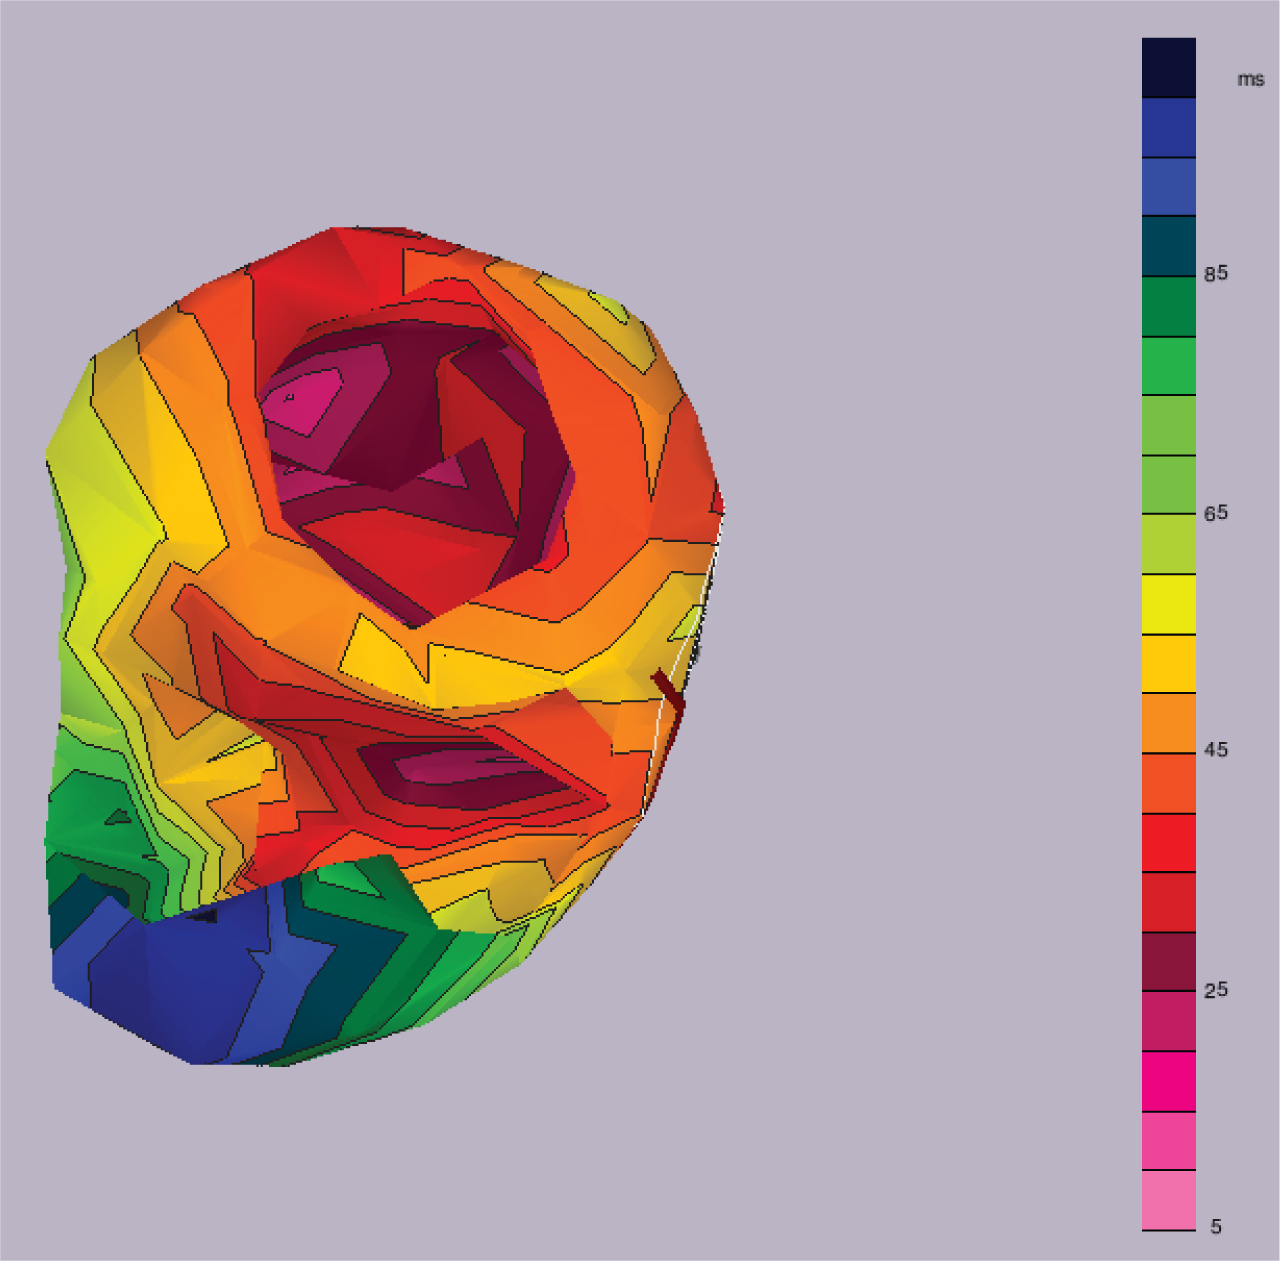
\includegraphics[width=.95\linewidth]{Figures/1_1_actTimes_1.png}
		\caption{}
		
	\end{subfigure}%
	\begin{subfigure}{.5\textwidth}
		\centering
		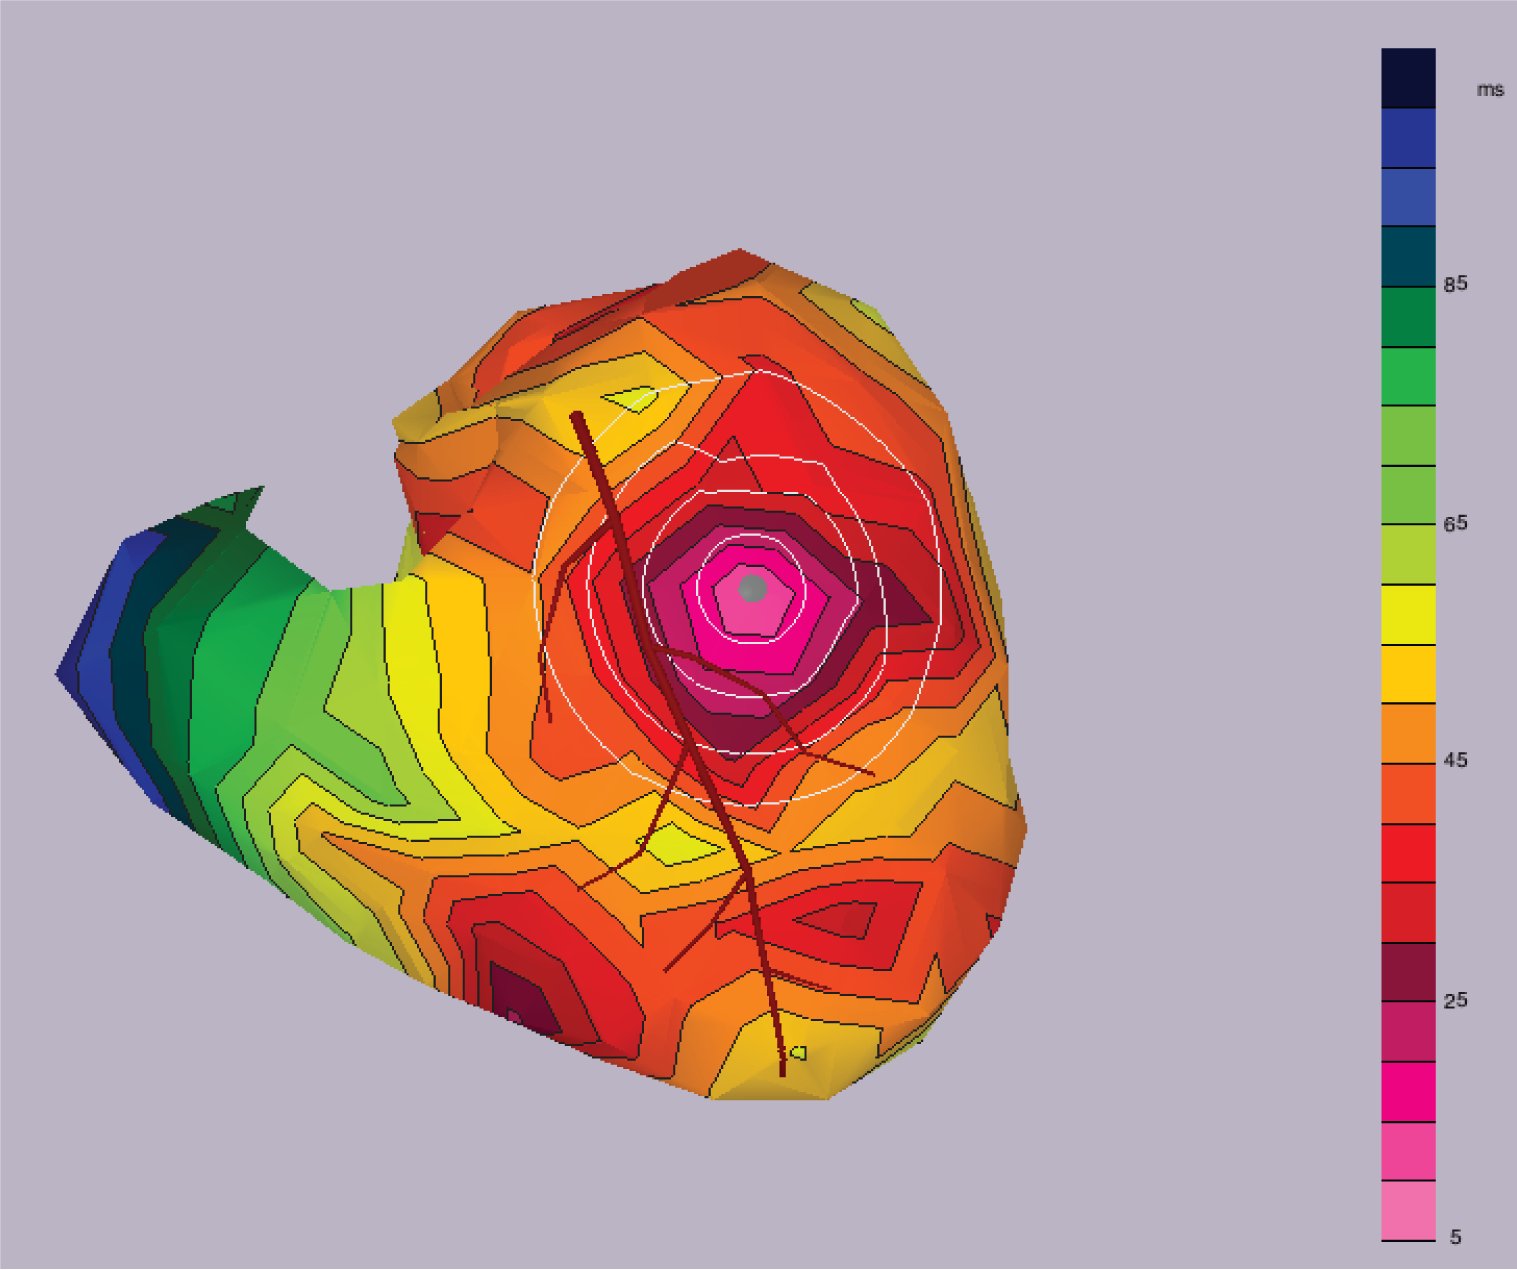
\includegraphics[width=.95\linewidth]{Figures/1_1_actTimes_2.png}
		\caption{}
		
	\end{subfigure}
	\caption{Activation times mapped onto the endocardium and epicardium. The color bar shows the spread of activation times. The heart is viewed from the atrial ventricular plane looking into the ventricles (a), and on the anterior surface (b).}
	\label{1_1_actTimes}
\end{figure}

\begin{figure}[H]
	\centering
	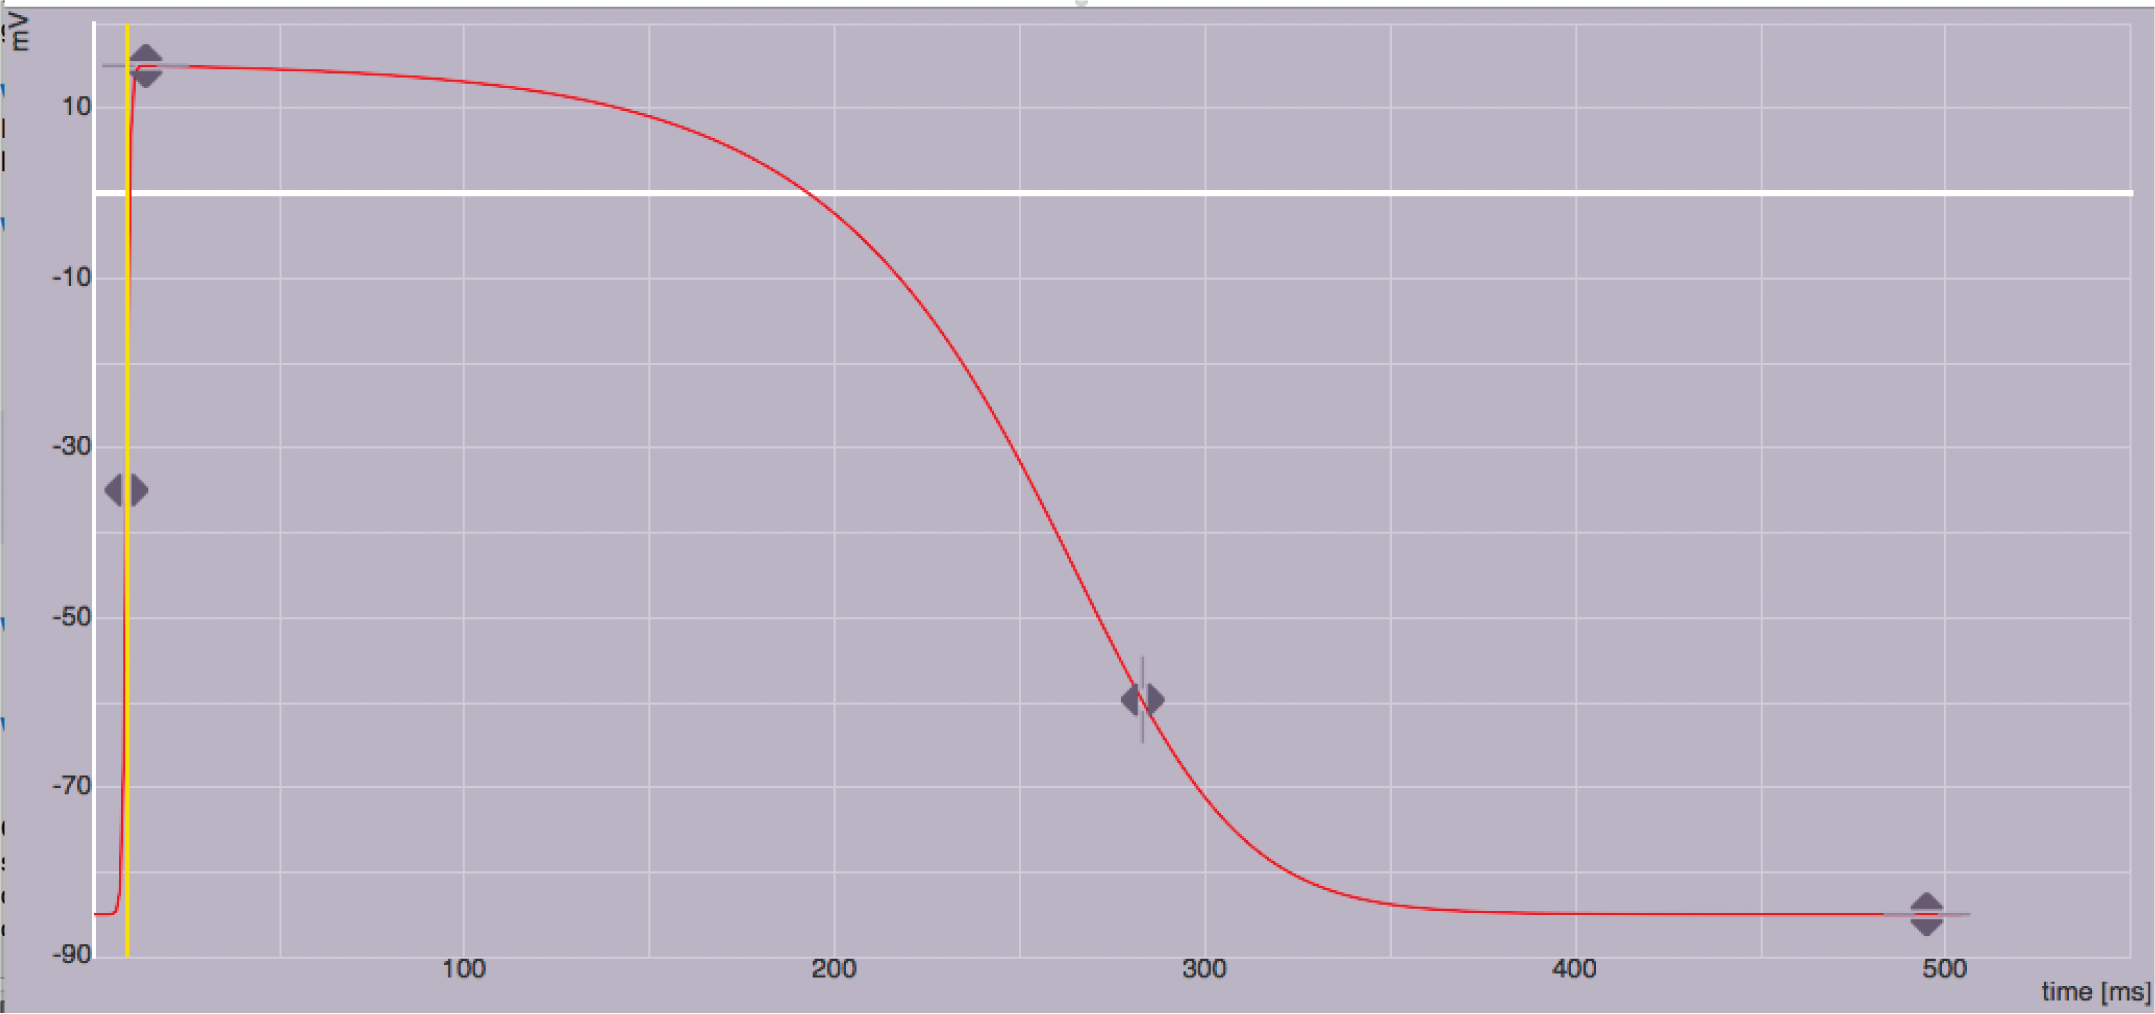
\includegraphics[width=.95\linewidth]{Figures/1_1_actpotential.png}

	\caption{Membrane potential of the node highlighted in Figure~\ref{1_1_actTimes}.b}
	\label{1_1_vm}
\end{figure}

\subsection{1.2: }
The pattern of deactivation or recovery is less ordered than that of activation. In the case of activation there is a wave of propagating depolarization of cells that drives neighboring cells to activate, and the wave properly propagates. In the case of recovery, each cell simply recovers at the end of its plateau phase, independent for the most part from its neighbors. Thus there is no explicit link between neighboring cells recovering. However, generally many myocytes have similar action potential duration, although this varies throughout the myocardium. Thus generally the last myocyte to activate is also the last to repolarize, and this is seen in Figure~\ref{1_2_recTimes} in which the right ventricular base is the last to recover. The recovery times range from 260 ms to 360 ms. The action potential of one region is shown in Figure~\ref{1_2_vm} with the time marker at the recovery time which is the time of steepest down slope of the repolarization phase of the action potential. The earlier sites of recovery are generally those that activated earlier but due to heterogeneity in action potential length this is not always true, as can be seen when comparing Figures~\ref{1_1_actTimes}~and~\ref{1_2_recTimes}.

\begin{figure}[H]
	\begin{subfigure}{.5\textwidth}
		\centering
		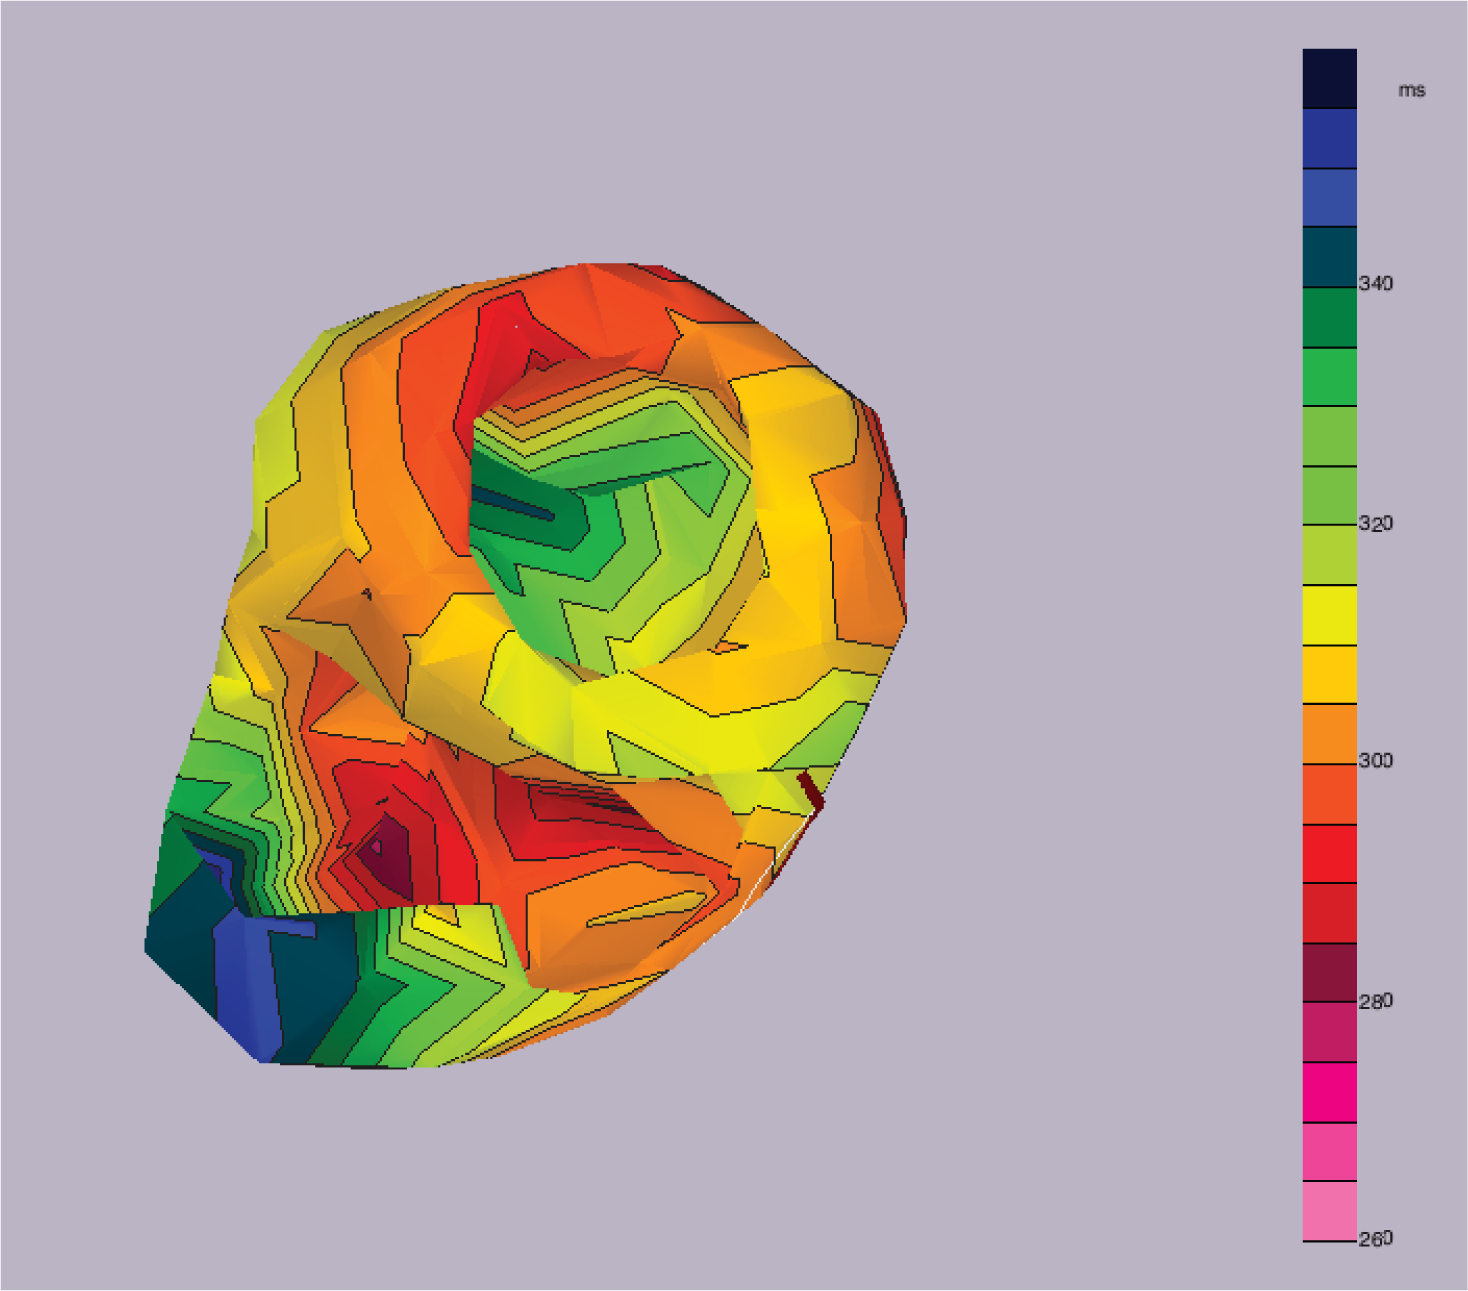
\includegraphics[width=.95\linewidth]{Figures/1_2_recTimes_1.png}
		\caption{}
		
	\end{subfigure}%
	\begin{subfigure}{.5\textwidth}
		\centering
		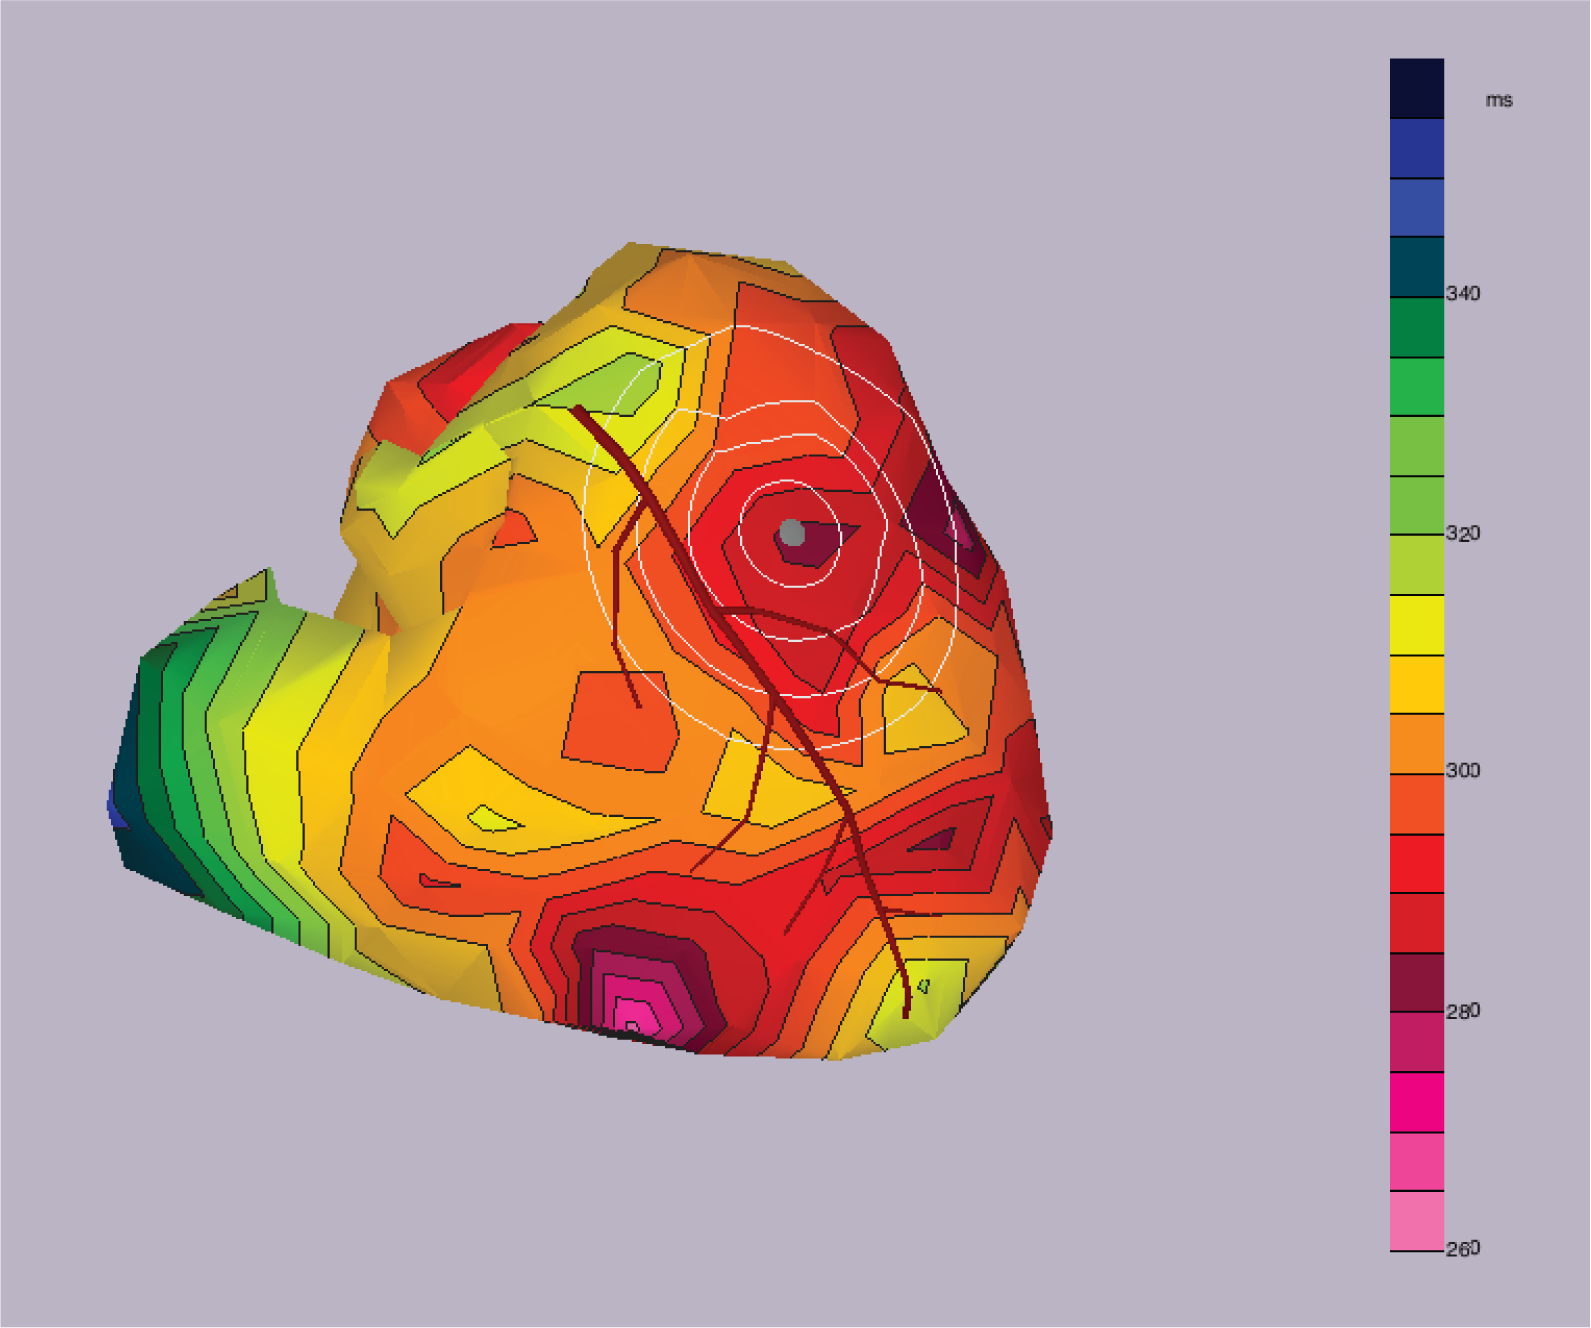
\includegraphics[width=.95\linewidth]{Figures/1_2_recTimes_2.png}
		\caption{}
		
	\end{subfigure}
	\caption{Recovery times mapped onto the endocardium and epicardium. The color bar shows the spread of recovery times. The heart is viewed from the atrial ventricular plane looking into the ventricles (a), and on the anterior surface (b).}
	\label{1_2_recTimes}
\end{figure}

\begin{figure}[H]
	\centering
	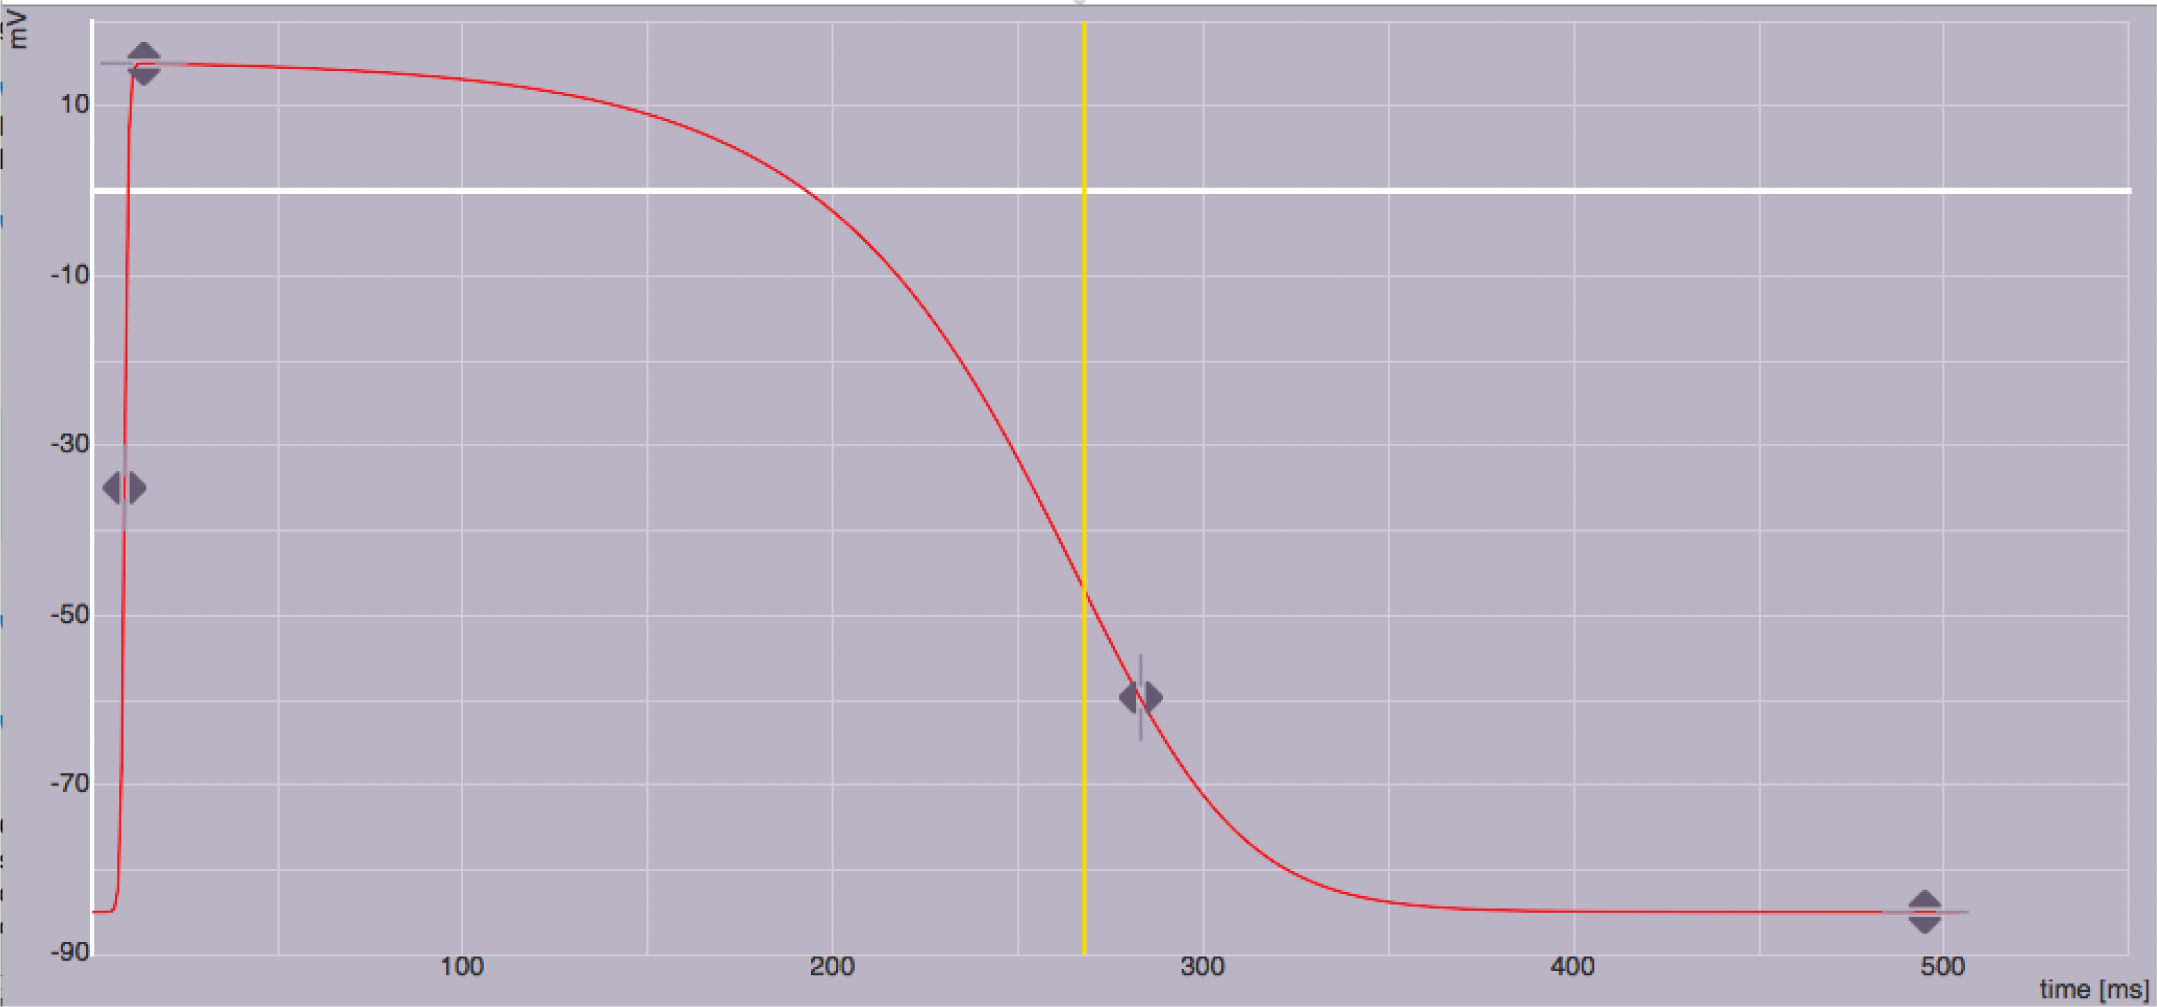
\includegraphics[width=.95\linewidth]{Figures/1_2_actpotential.png}
	
	\caption{Membrane potential of the node highlighted in Figure~\ref{1_2_recTimes}.b}
	\label{1_2_vm}
\end{figure}


\subsection{1.3: }
The peak of extrcellular potential on the heart surface occurs during the QRS as seen on the ecg (Figure~\ref{1_3_1}). During this time the extracellular voltage ranges from about -35 mV to 35 mV. During the QRS there is a veyr high gradient of potentials along the heart surface, propagating wave of activation passes through the tissue. During this time there is a large intracellular and reciprocal extracellular potential gradient between the activated and unactivated tissue, particularly at the wavefront where some cells have just been activated and neighboring cells have yet to be activated. One such time instance is shown in Figure~\ref{1_3_2}. The highlighted tissue has yet to be activated while the tissue immediately surrounding it has been, resulting in a large potential gradient in this area.

\begin{figure}[H]
	\begin{subfigure}{.75\textwidth}
		\centering
		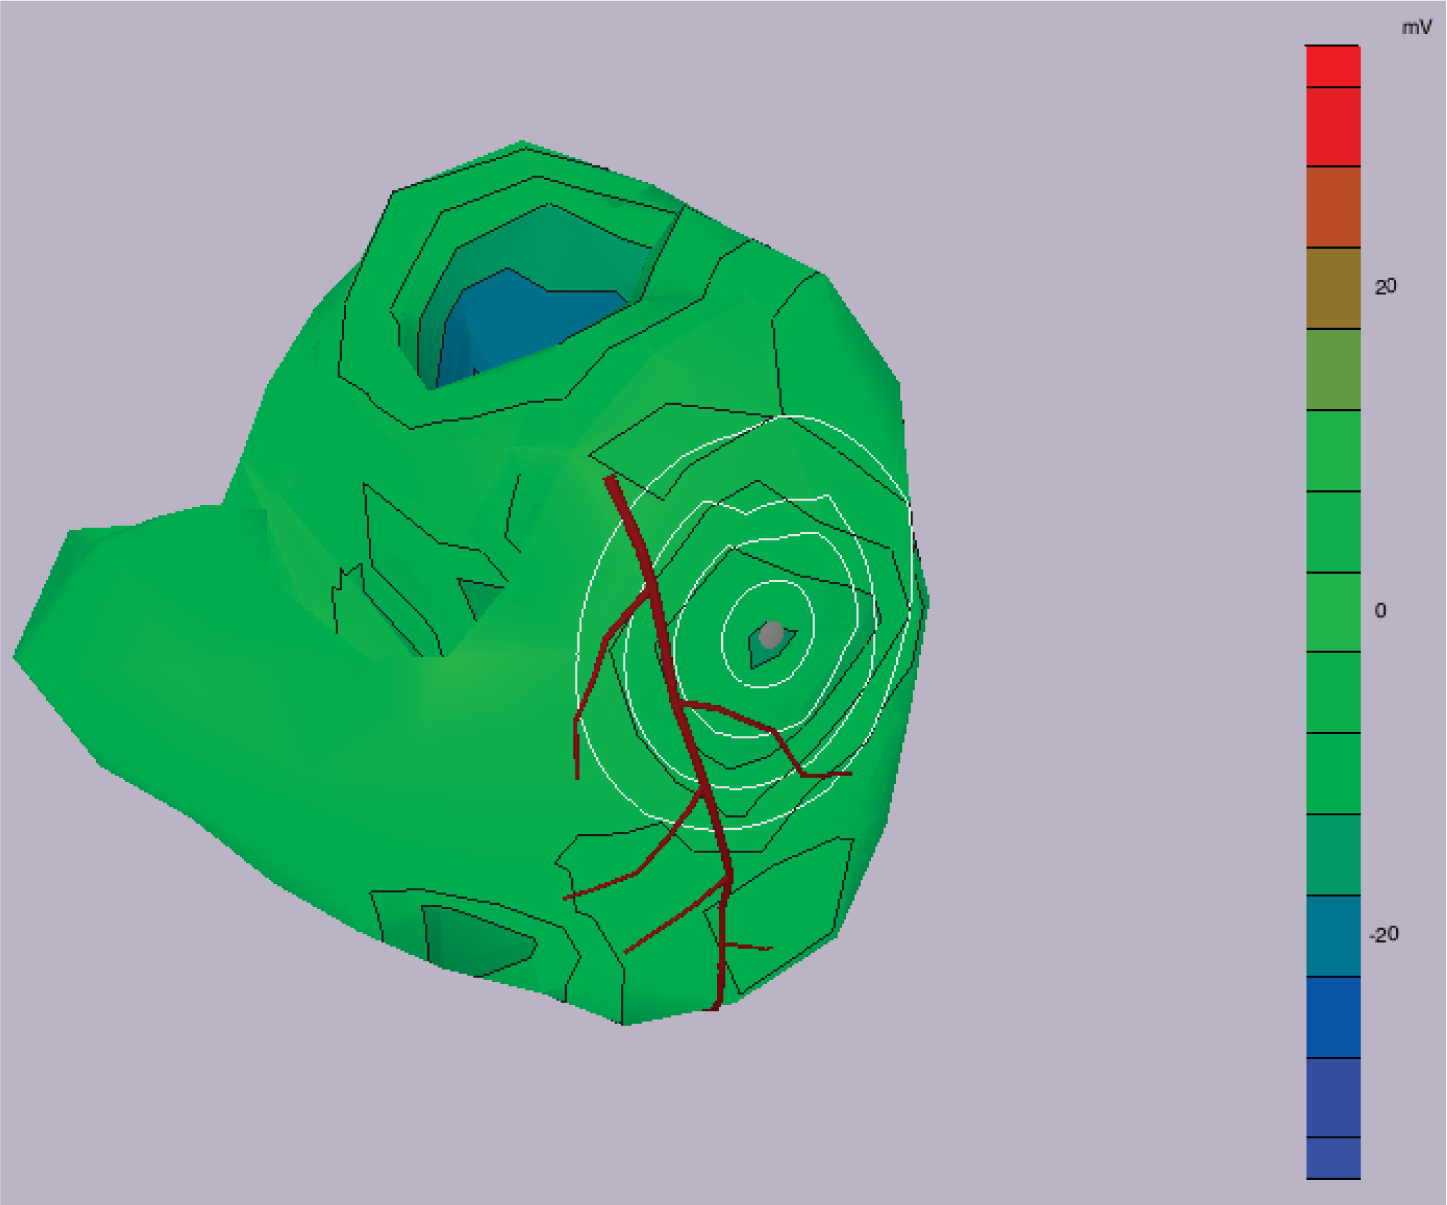
\includegraphics[width=.95\linewidth]{Figures/1_3_pot_1.png}
		\caption{}
		
	\end{subfigure}%
\\
	\begin{subfigure}{.95\textwidth}
		\centering
		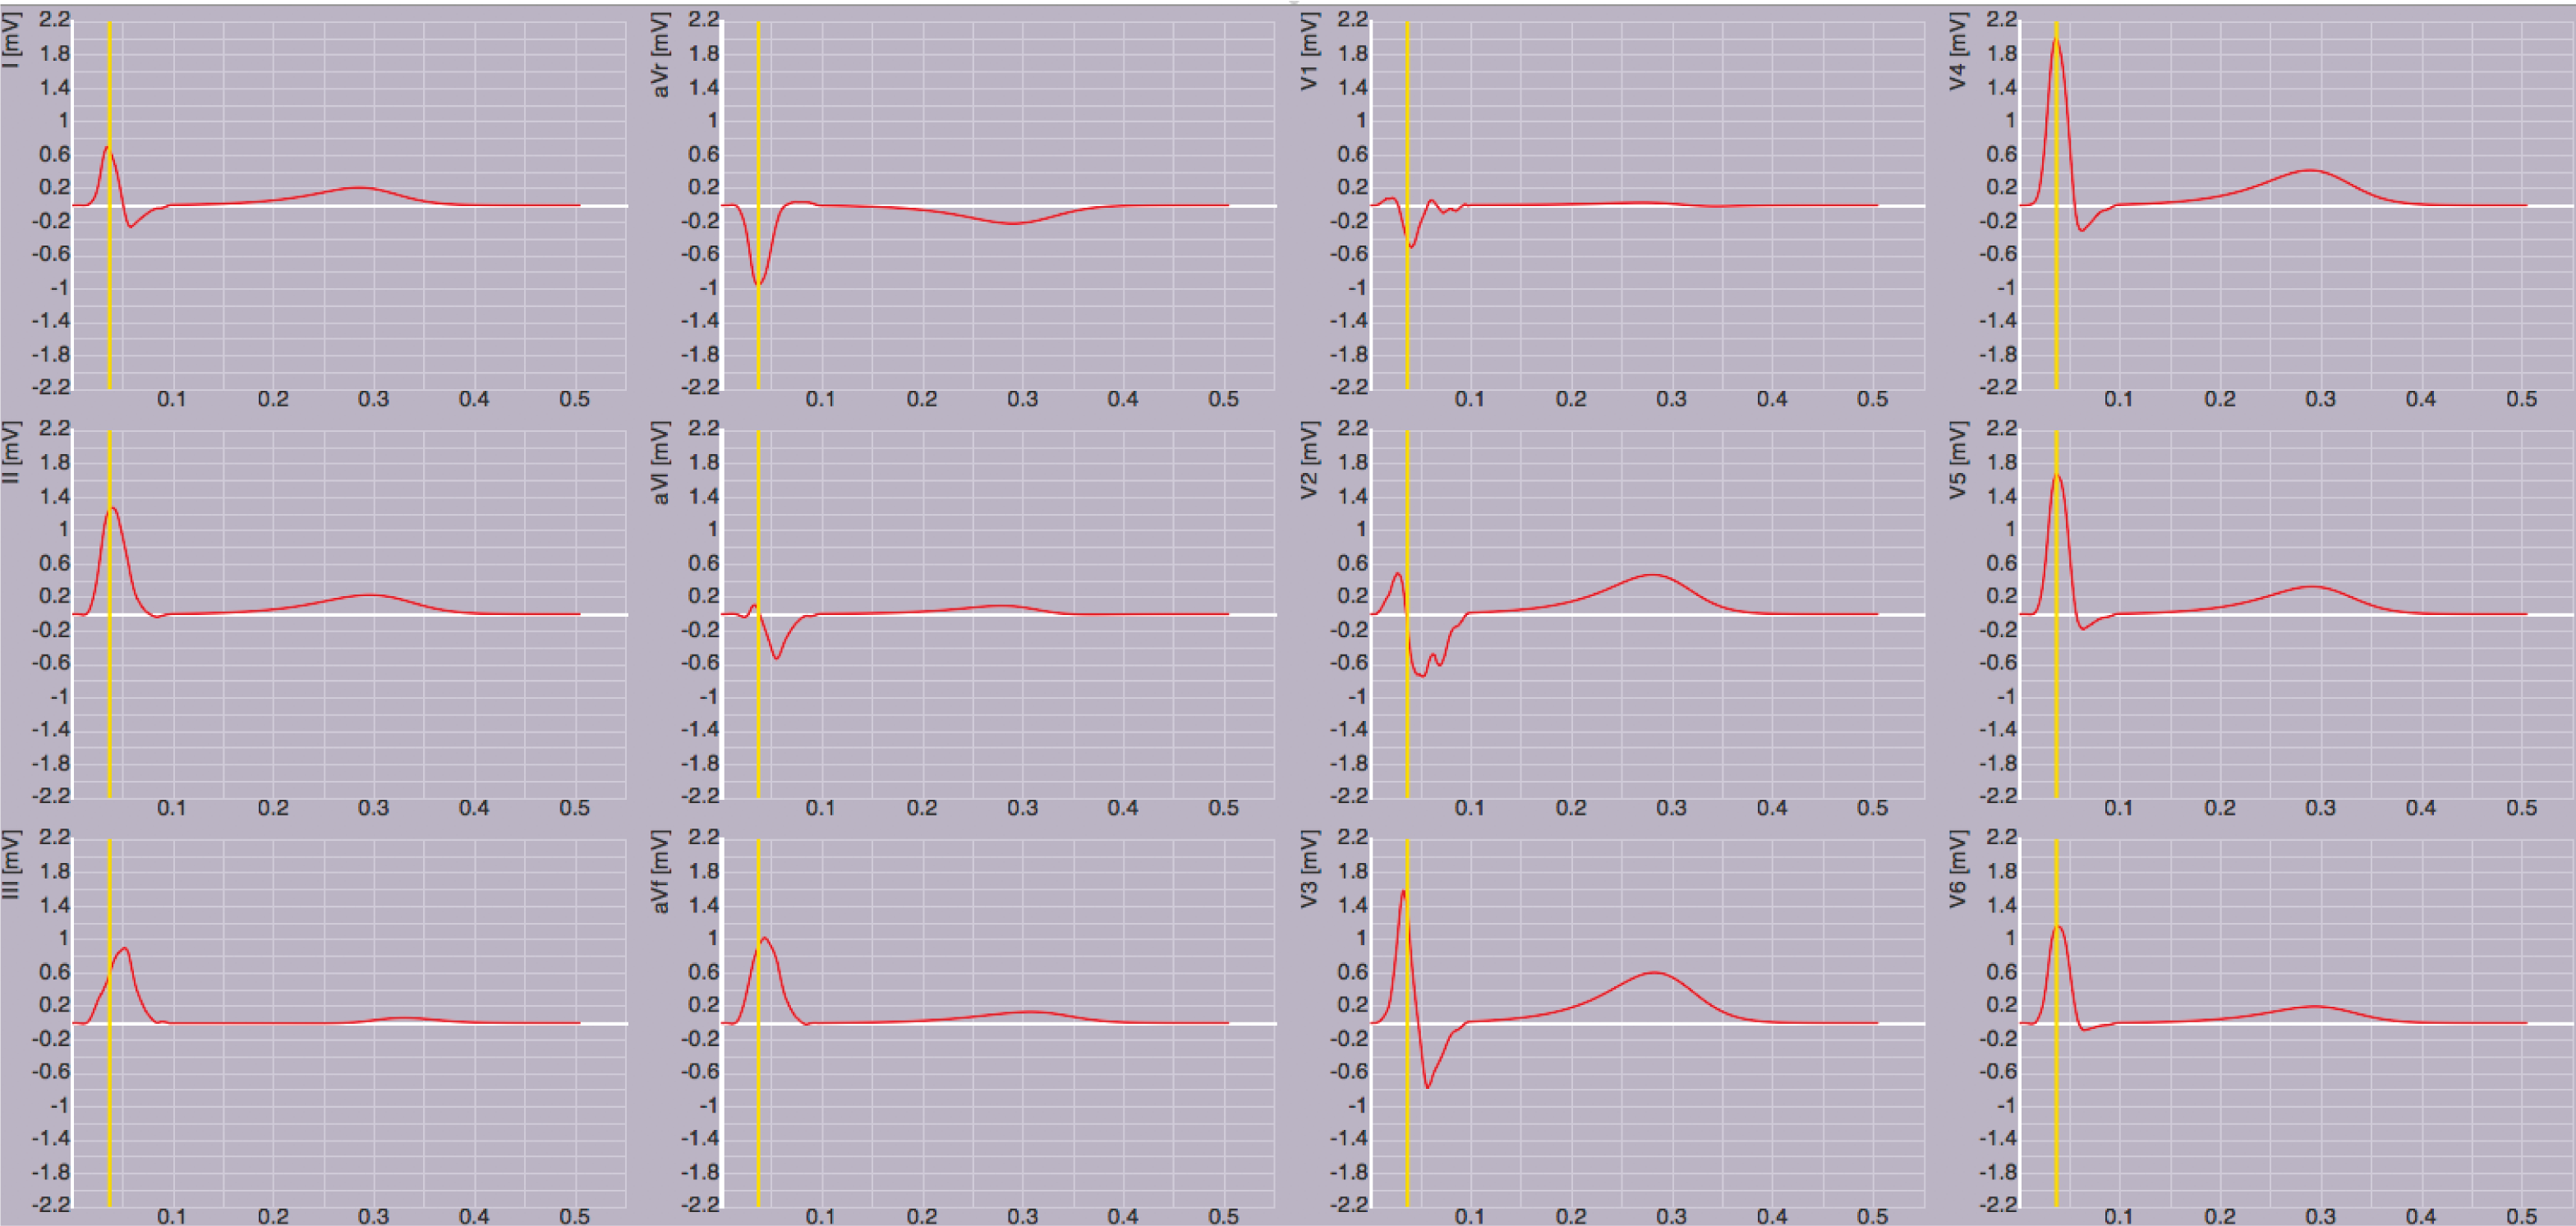
\includegraphics[width=.95\linewidth]{Figures/1_3_ecg_1.png}
		\caption{}
		
	\end{subfigure}
	\caption{Extracellular potentials mapped onto the epicardium and endocardium during peak extracellular voltage (a), and the associated ECG signals (B).}
	\label{1_3_1}
\end{figure}
\begin{figure}[H]
	\begin{subfigure}{.75\textwidth}
		\centering
		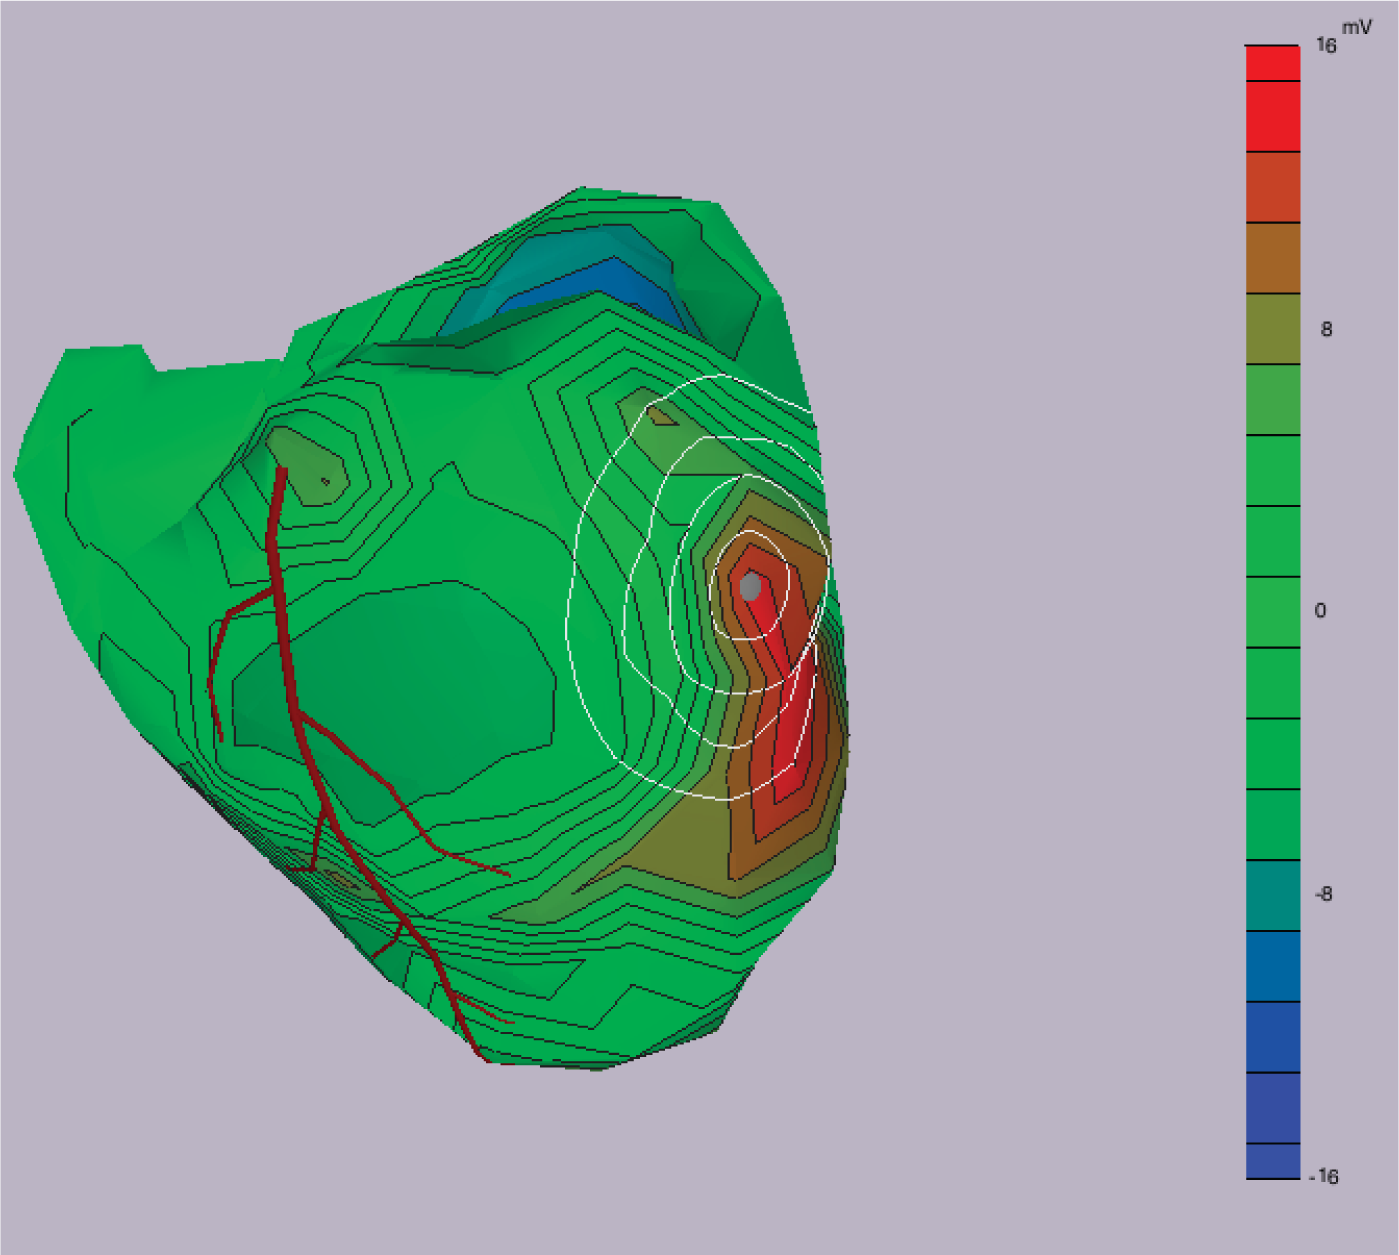
\includegraphics[width=.95\linewidth]{Figures/1_3_pot_2.png}
		\caption{}
		
	\end{subfigure}%
\\
	\begin{subfigure}{.95\textwidth}
		\centering
		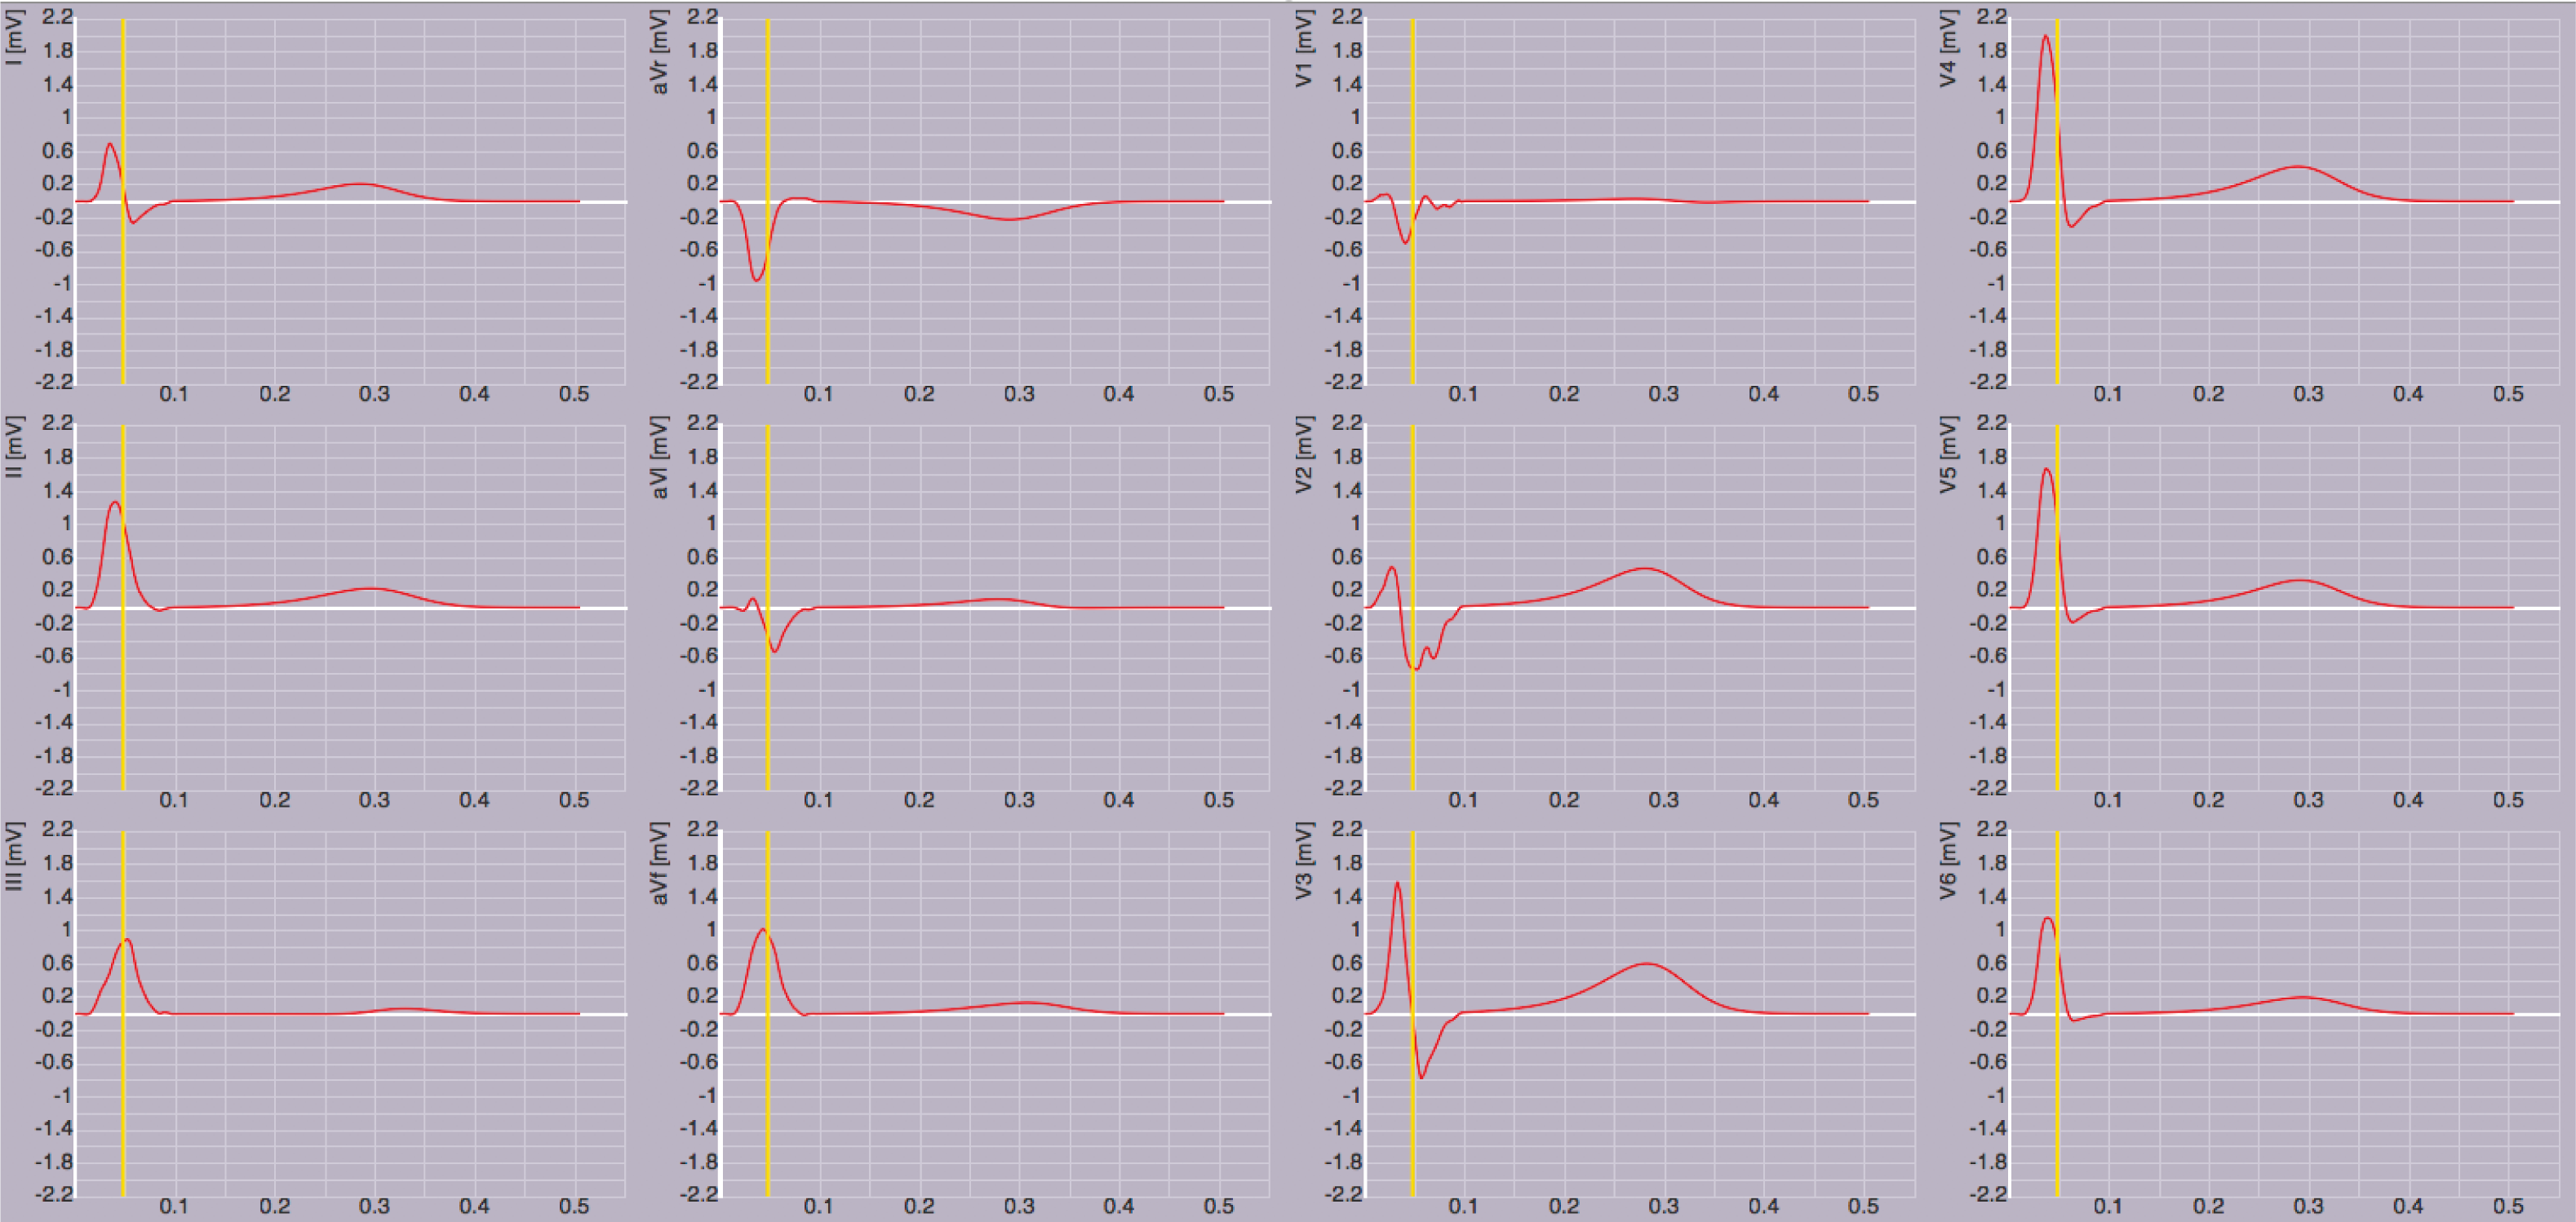
\includegraphics[width=.95\linewidth]{Figures/1_3_ecg_2.png}
		\caption{}
		
	\end{subfigure}
	\caption{Extracellular potentials mapped onto the epicardium and endocardium during a timeoint wiht large extracellular potential gradient on the epicardium (a), and the associated ECG signals (B). The hilighted node is one that has yet to activate surrounded by nodes that have just activated.}
	\label{1_3_2}
\end{figure}


\subsection{2.1: }
In a clinical ECG 12 ``leads'' are used. In actuality only 9 electrodes are placed on the body (the three limb leads and the 6 precordial leads) while the remaining leads are computed mathematically from the limb leads and represent theoretical measurement locations on the torso (aVr, aVl, aVf). The three limb leads are placed to form Einthoven's triange, an ``equlatteral'' (mostly) triangle of leads placed on the right and left arms and the left leg. In practice and in this simulation dataset these leads are placed actually on the torso ont he right and left shoulder, and the left lower abdomen. This is an acceptable approximation of placing them on the limbs as the limbs are considered to be passive conductors. Three bipolar recordings are made across these leads as described int he introduction, resulting in leads I, II, and III of the ECG. The precordial leads are unipolar recordings, whose reference is Wilson's central terminal. Wilson's central terminal is constructed by feeding the three limb lead electrodes through equal resistors into one terminal, averaging their potentials an creating a reference that represents something like a center of the chest reference point or plane. This allows the precordial leads (V1-V6) to record local activity from the heart almost as if the vector of recording projected from the center of the heart to the precordial electrode. The augmented leads are calculated using the limb leads. By averaging two of the limb lead electrodes through resistors and constructing a bipolar recording from this averaged ``electrode" to the third limb lead the augmented leads are made and represent recording vectors that bisect the sides of Einthoven's triangle. The aVf is constructed from -(RA LA) + LL, aVr from -(RA LL) +LA, and aVl from -(LA LL) +RA, where RA is right arm, LA is left arm, LL is left leg, + is the postive pole of the recording, - is the negative and ( ) is the average of two leads.

In the case of ECG sim, the body surface potentials displayed represent unipolar recordings with respect to a reference such as Wilson's central terminal. Thus the bodysurface potentials can be used to reconstruct the 12 lead ECG signals as described above. The limb lead potentials are subtracted from eachother to form bipolar recordings according to the lead I, II, and III arrangements. the aVf, aVl, and aVr recordings are constructed from the limb lead potentials. The precordial recordings can be taken as is from their mesh locations or constructed by subtracting Wilson's central terminal voltage from each potential at the precordial locations. (Note: if the bodsy surface poteitnals simulated are referenced to a reference like Wilson's central terminal, then the Wilson's central terminal value for these body surface ptoentials should be zero and the precordial lead signals can be taken as they are.) The locations of the precordial and limb lead electrodes in ECG sim are shown in Figure~\ref{2_1}. Arrows indicate the locations of the difficult to see limb lead electrode markers. The voltage range for the typical ECG signals is roughly -1 mV to 2 mV. Because this simulation lacks atrialactivity there is a distinct lack of a P wave in the ECG signals due to a lack of atrial activation signals. The remaining typical ECG waveforms (QRS complex, and T wave) are present in that order. Additionally under normal circumstances the ST segment is near isoelectric as are the periods before the QRS and after the T wave.

\begin{figure}[H]
	\begin{subfigure}{.95\textwidth}
		\centering
		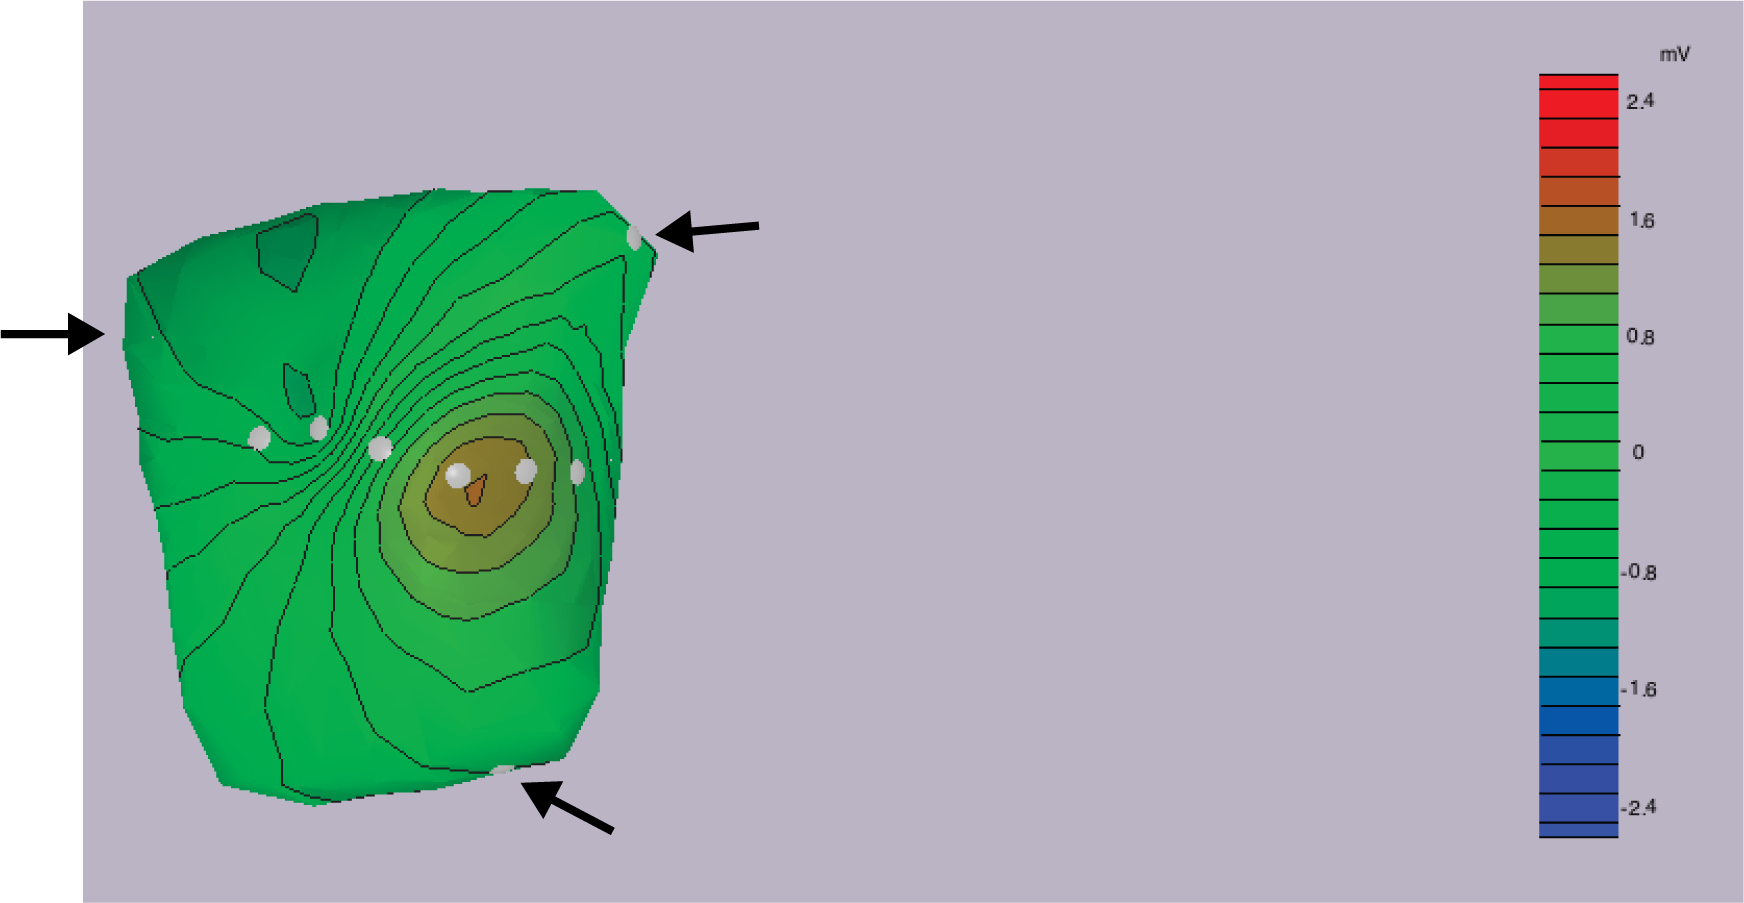
\includegraphics[width=.95\linewidth]{Figures/2_1_bsp.png}
		\caption{}
		
	\end{subfigure}%
	\\
	\begin{subfigure}{.95\textwidth}
		\centering
		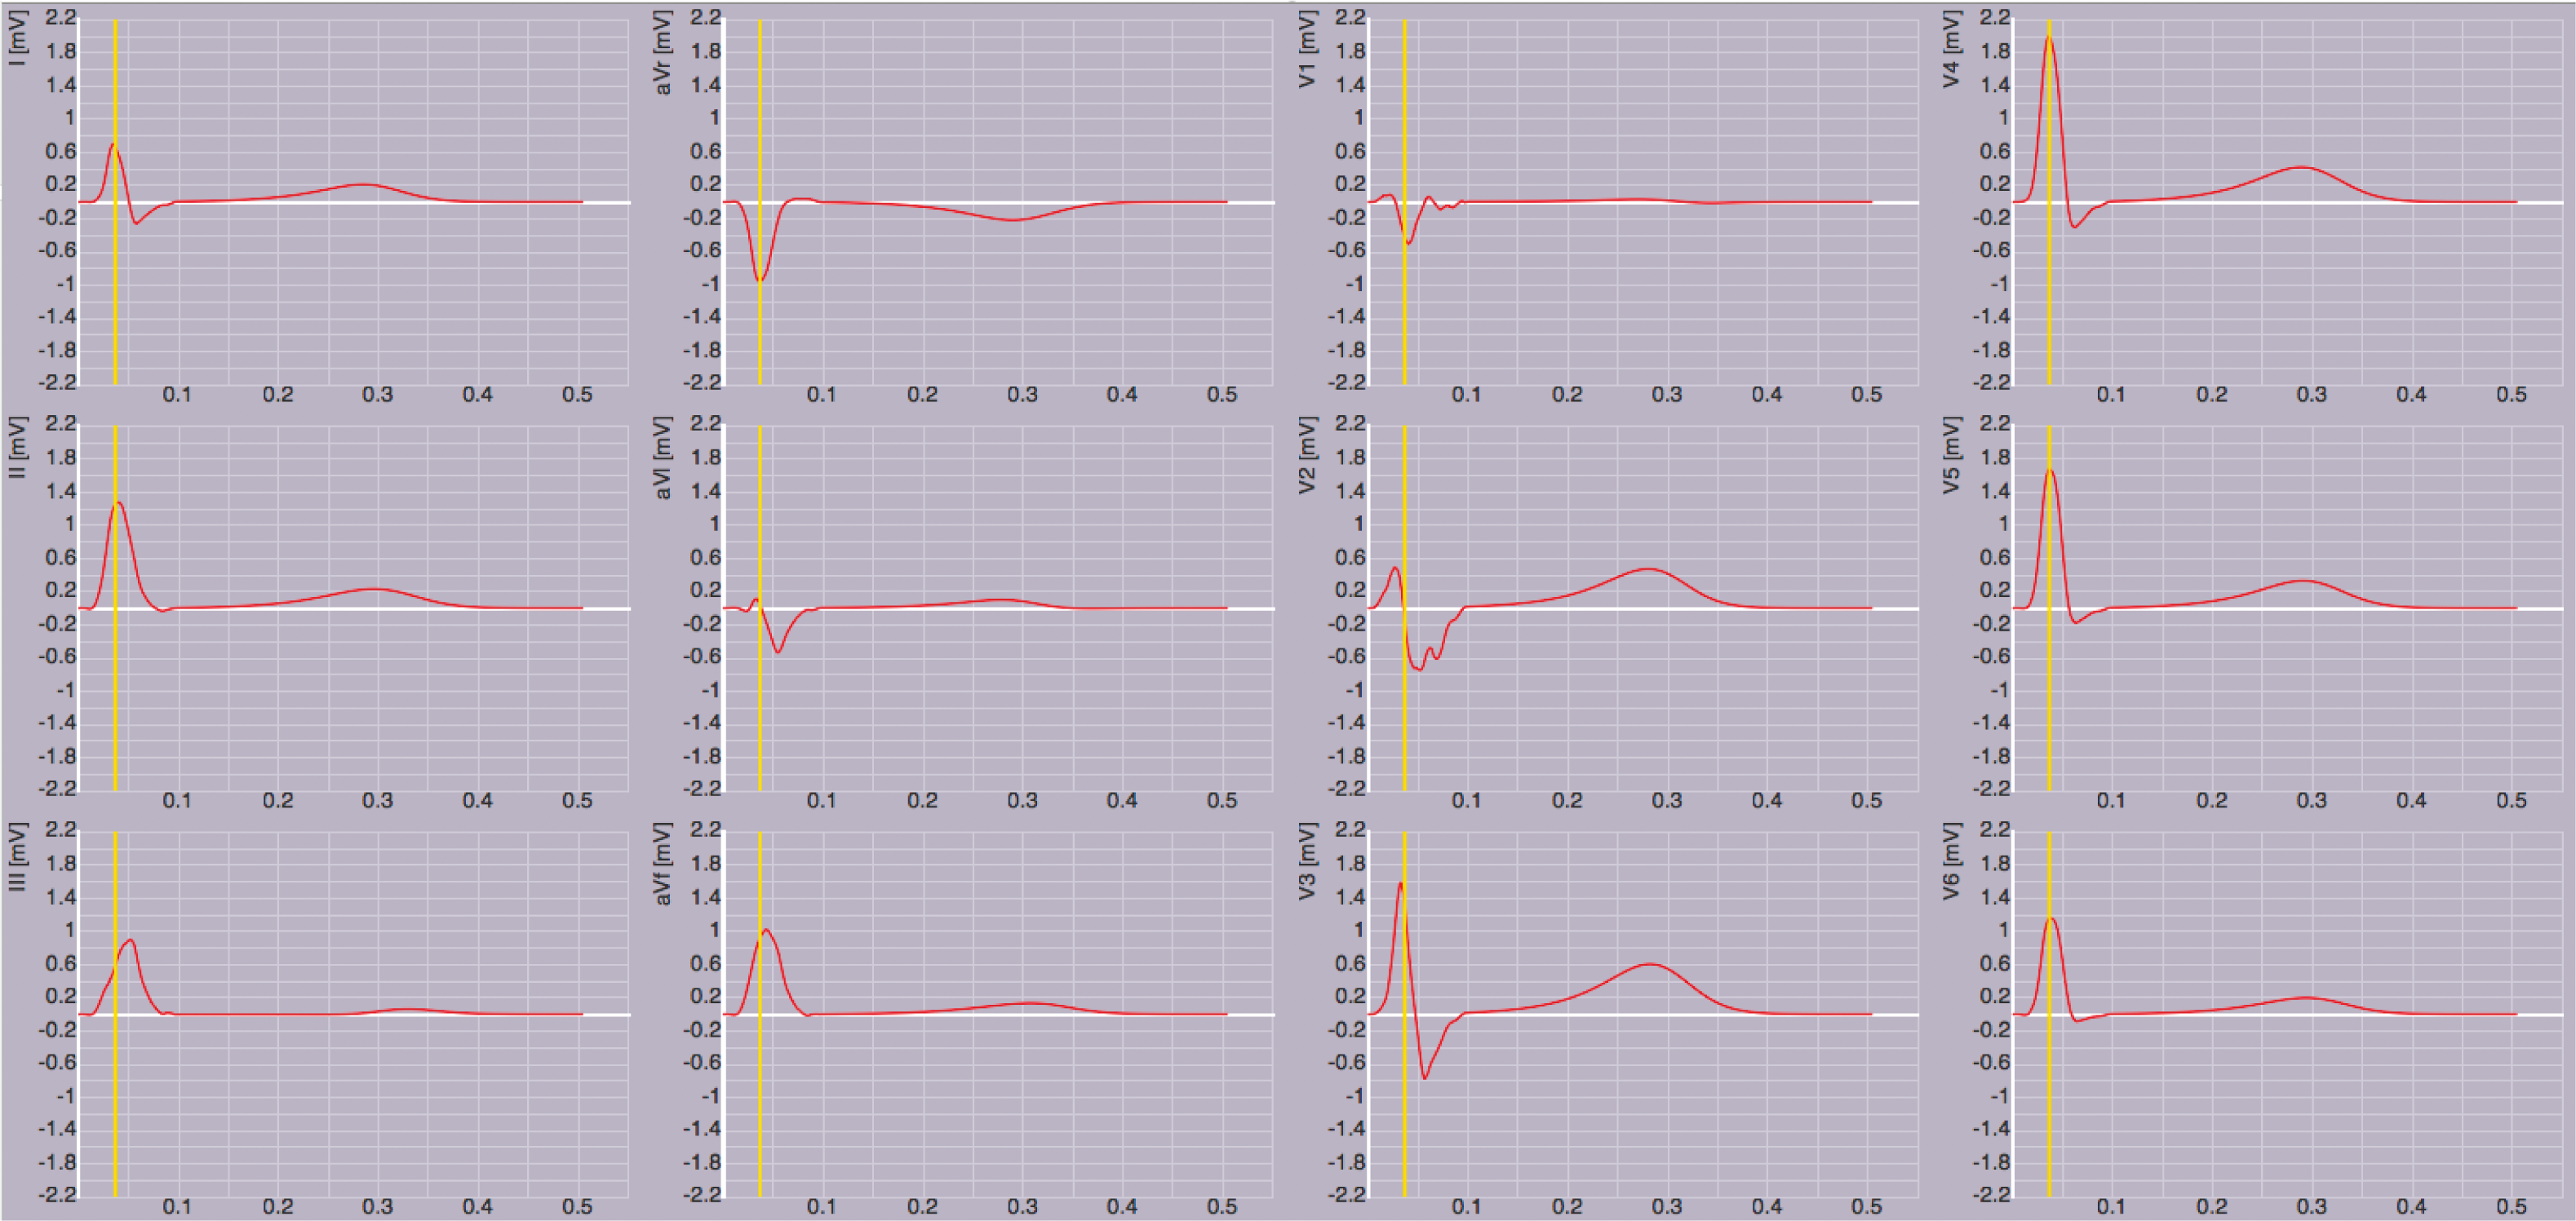
\includegraphics[width=.95\linewidth]{Figures/2_1_ecg.png}
		\caption{}
		
	\end{subfigure}
	\caption{The body surface potential map with 12 lead recording locations highlighted by white dots (a), and the associated ECG signals (b). Black arrows indicate the locations of the limb leads.}
	\label{2_1}
\end{figure}


\subsection{2.2: }
Because this segment deals with alterations to the action potential length, visualizing activation recovery interval (ARI) should be an appropriate way of assessing changes to action potential length spatially. The baseline ARI across the heart is shown in Figure~\ref{2_2_base} with the node of interest int he left ventricle highlighted. By lengthening the action potential duration by roughly 25\% (from ~250 ms to ~312 ms) as shown in Figure~\ref{2_2_25}.b the resulting ARI map and ECG are produced as seen in Figure~\ref{2_2_25}. Because the changes made did not affect activation the QRS complex remains the same for all leads. These changes should change the T wave morphology as the are of the action potnetial affected is the plateau and recovery phase, those associated with the T wave. Looking at lead I particularly we can see that the T wave has been delayed, as would be expected by a delay in recovery resulting from prolonged action potentials. The only lead that does not see this phenomena is V1, which makes sense given that V1 records activity primarily from the right ventricle which had no changes, and the are of the left ventricle that chaged would result in aT wave perpendicular to the axis of V1 recording, thus it would be blind to these changes. Again looking back to lead I we also see a slight depression before the T wave. 

If we increase the duration from 25\% increase to a 50\% increase (~375 ms) we see the same trends as before but more emphasized (Figure~\ref{2_2_50}). The T wave of lead I is later and now has a higher amplitude and is preceeded by a slight depression. The higher aplitude is likely due to the fact that now when the left ventricle is repolarizing, most of the rest of the heart has already repoarized and the only activity at that time is the left ventricular repolaization. Thus there is no destrctive interfereance of potentials projecting onto the lead I vector as the left ventricular repolarization ``wavefront" (not a real wave but sequence of repolaization events) is well aligned with lead I. The depression is likely a symptom of the same, where during the early phases of repolarization the left ventricle has not started to repeolarize but the rest of the heart is, and the general repolarization vector points slightly opposite the direction of lead I, resulting in a slight negative potential registered by lead I.

\begin{figure}[H]
	\centering

	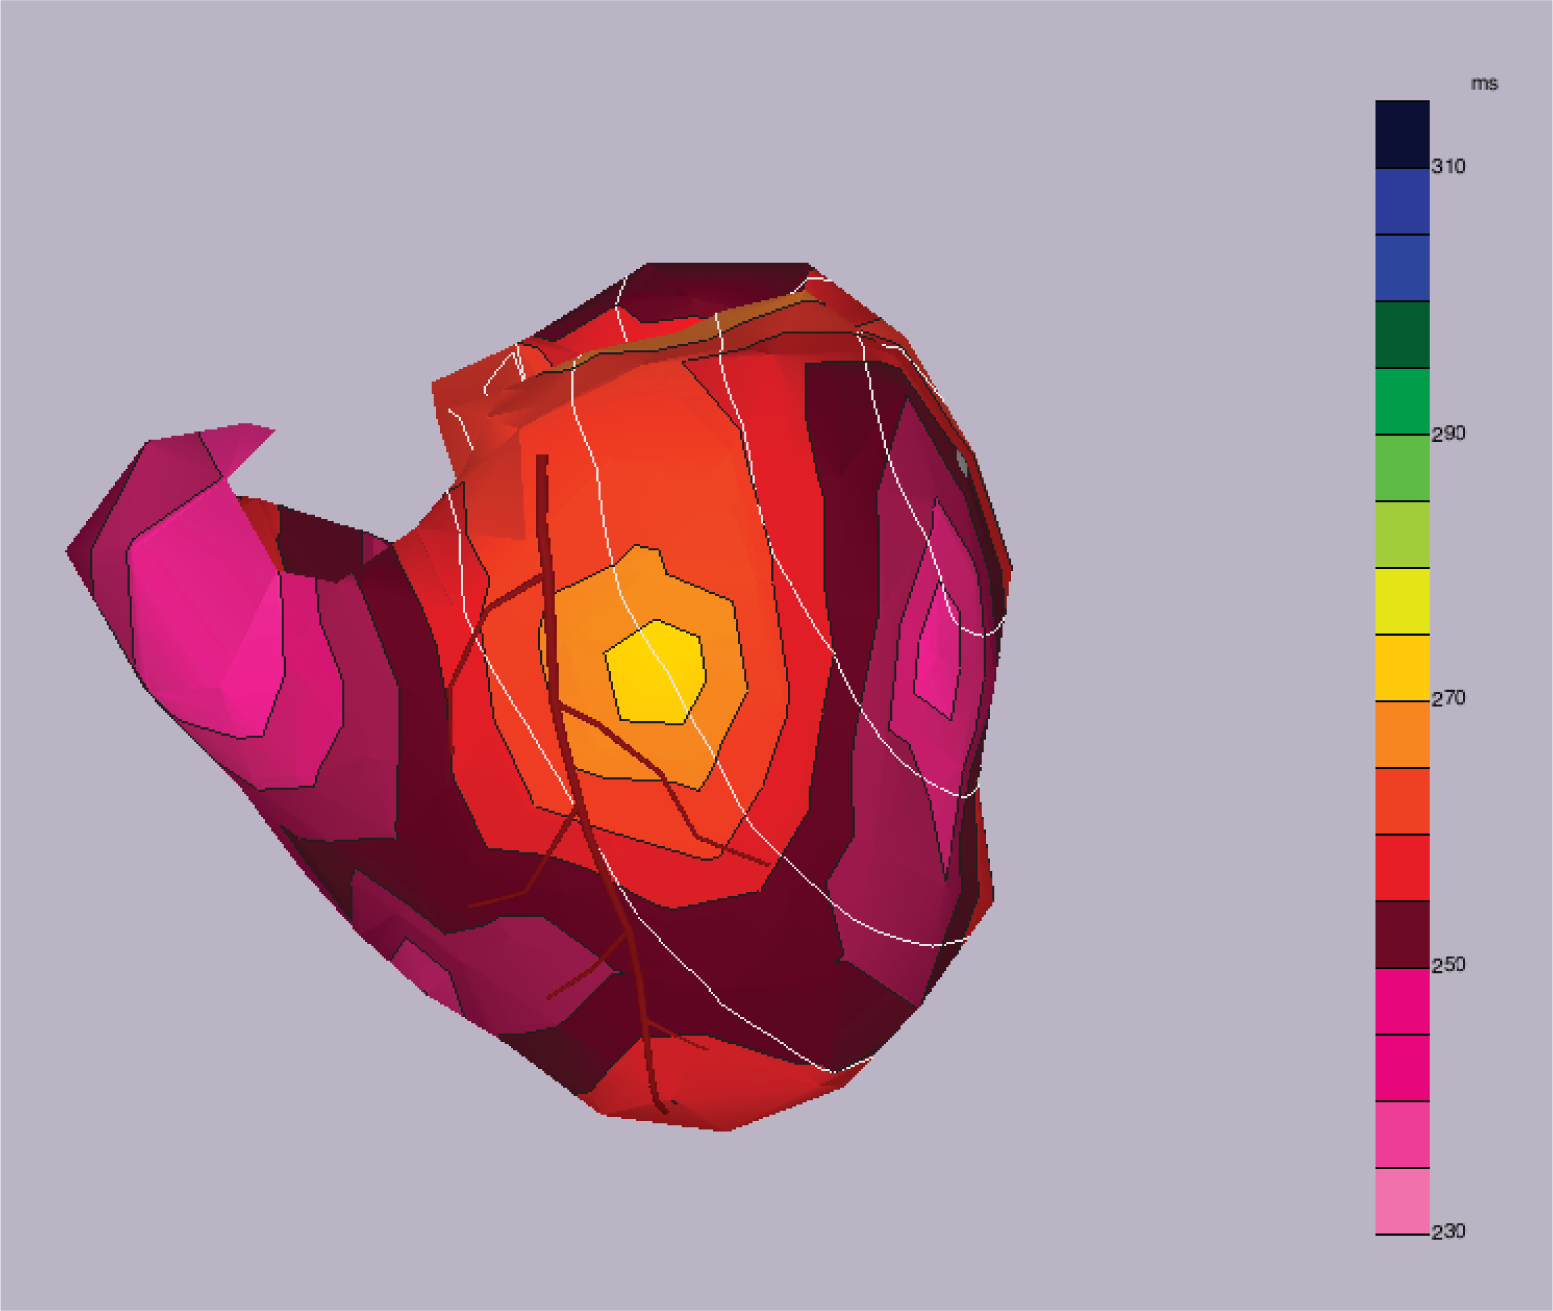
\includegraphics[width=.5\linewidth]{Figures/2_2_baseARI.png}

	\caption{Default activation recovery interval mapped onto the heart surface. The highlighted node is the one whose action potential duration will be varied.}
	\label{2_2_base}
\end{figure}

\begin{figure}[H]
	\begin{subfigure}{.5\textwidth}
		\centering
		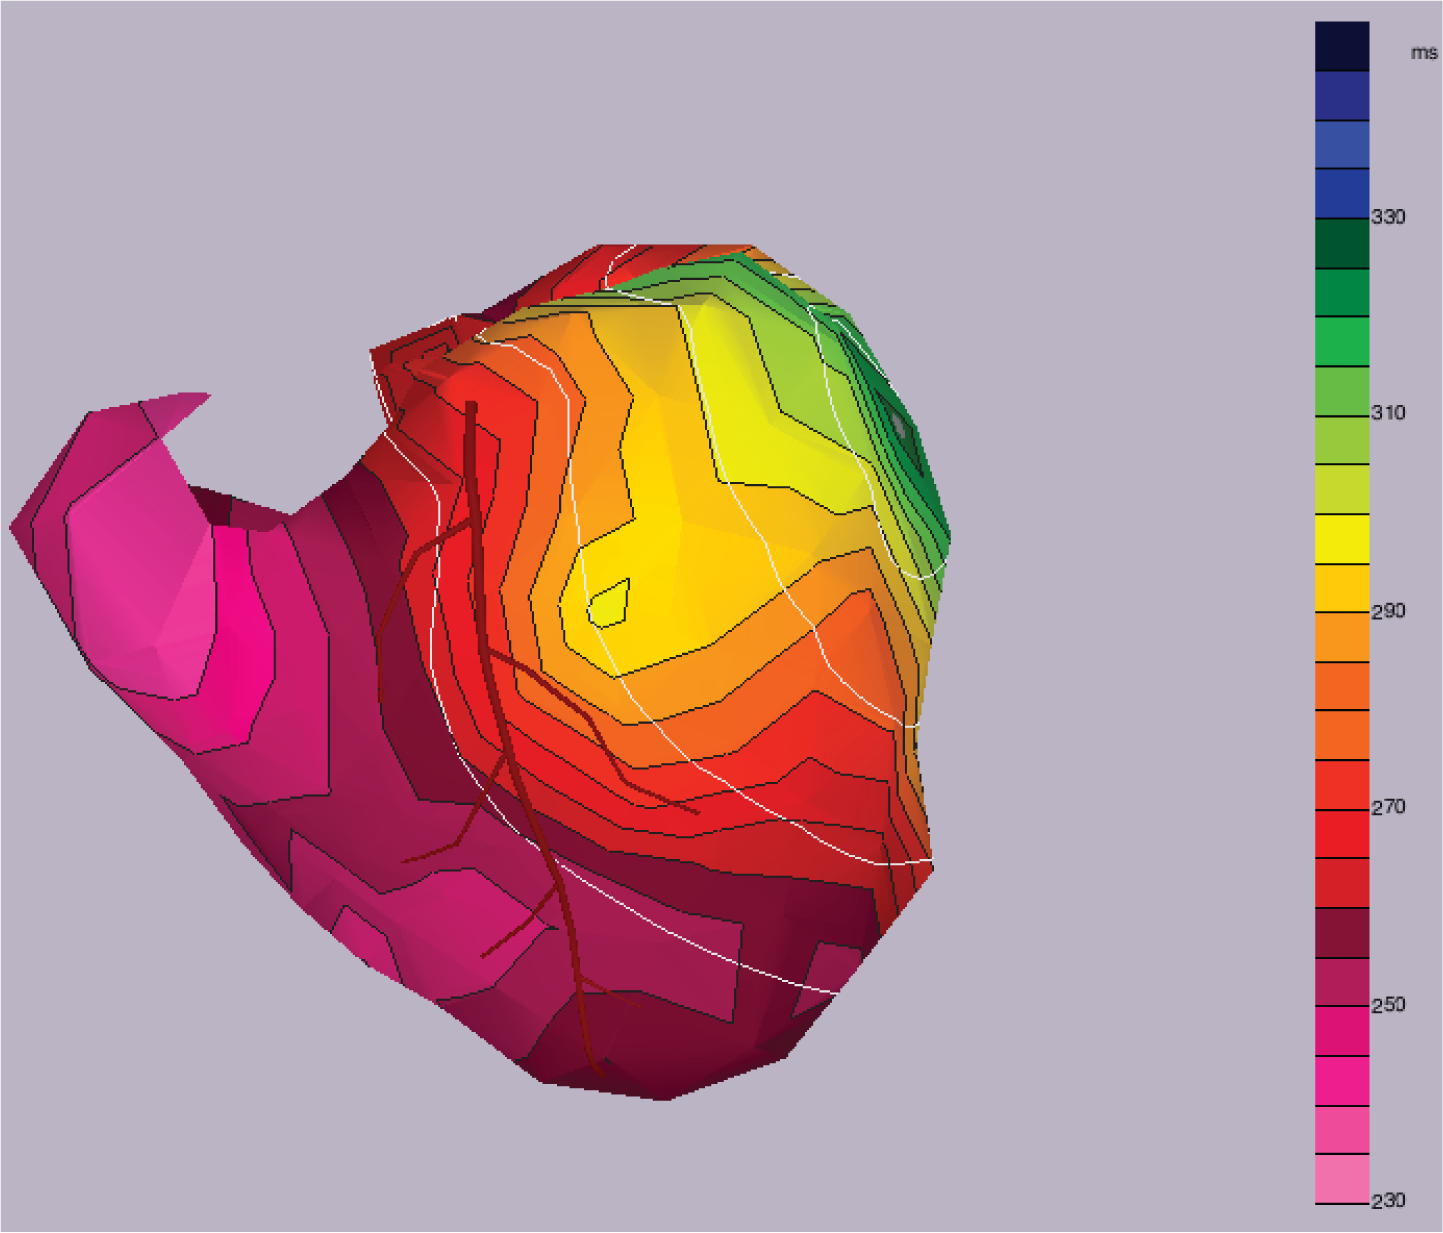
\includegraphics[width=.95\linewidth]{Figures/2_2_25ARI.png}
		\caption{}
		
	\end{subfigure}%
	\begin{subfigure}{.5\textwidth}
		\centering
		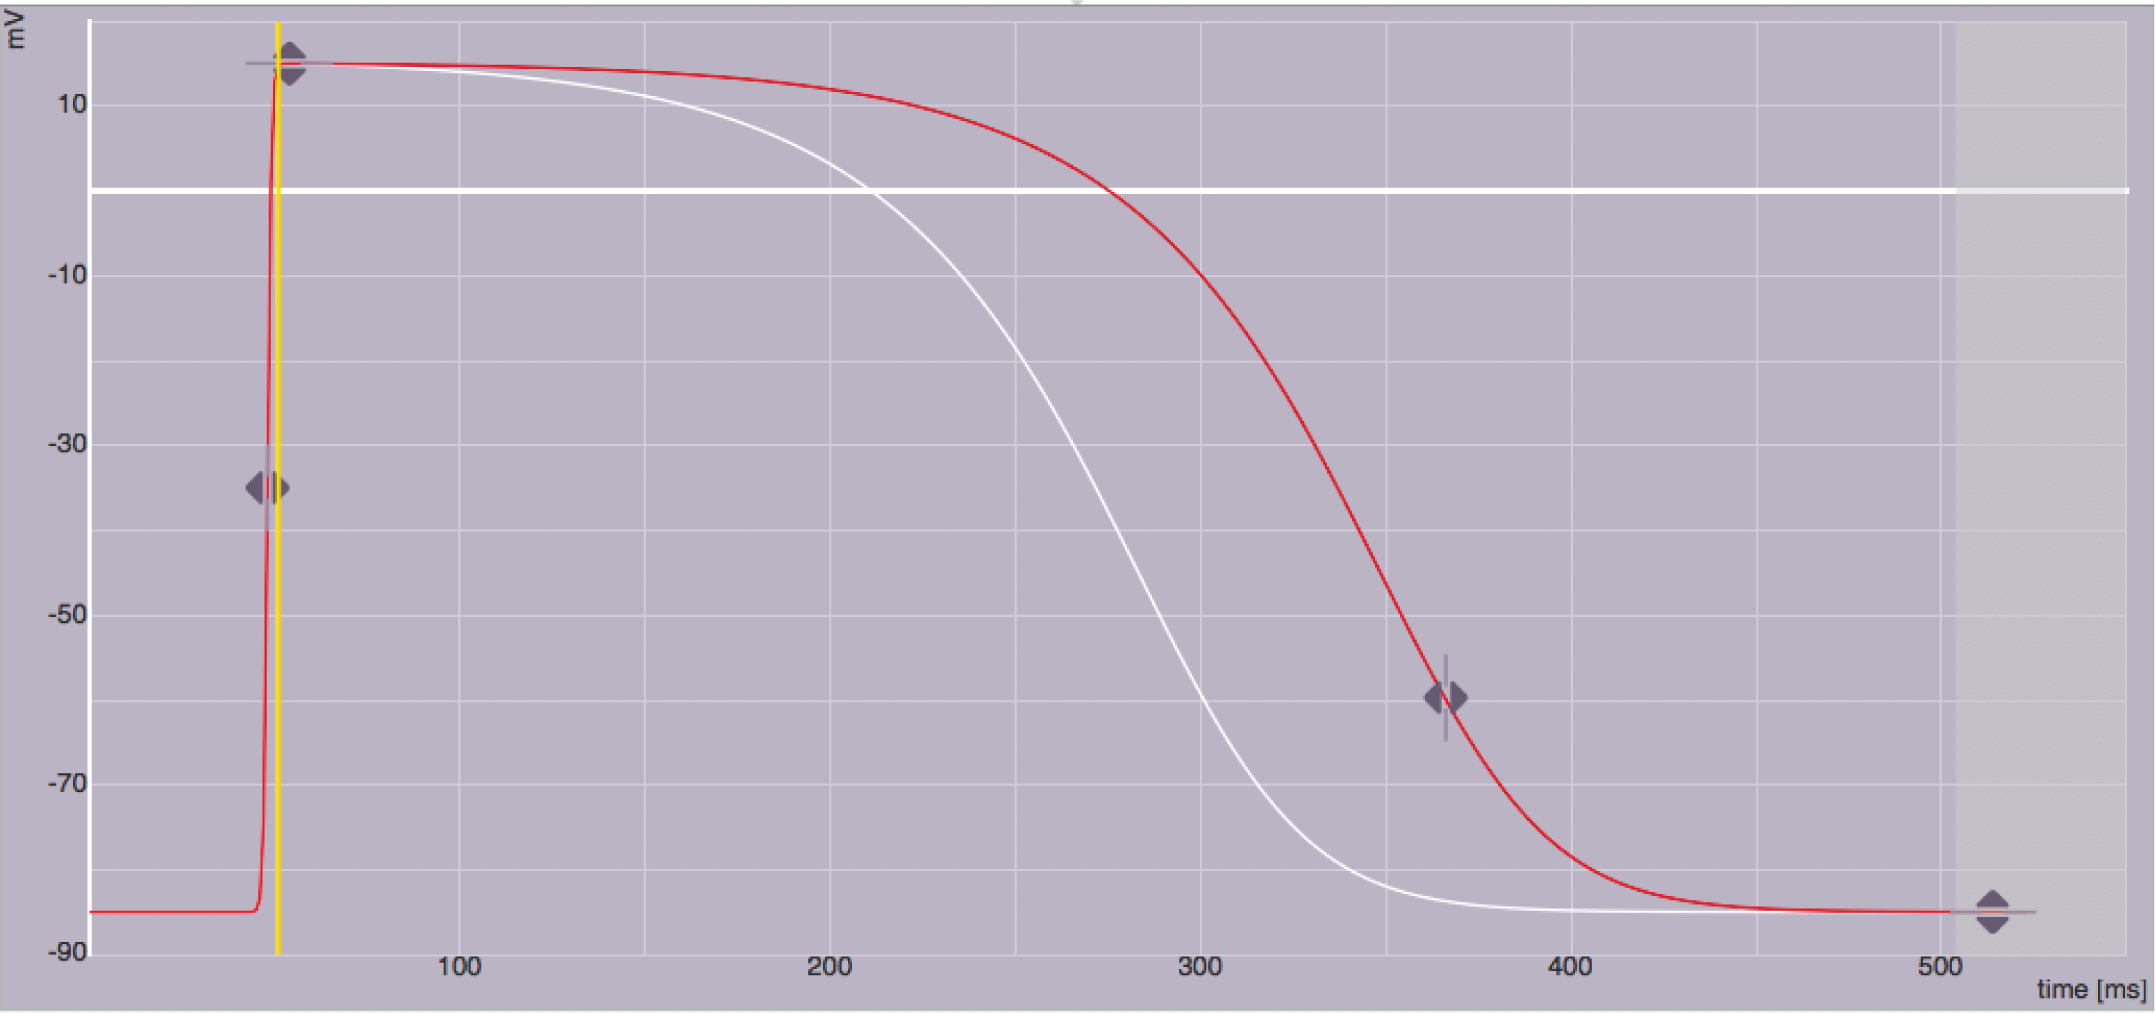
\includegraphics[width=.95\linewidth]{Figures/2_2_25Actionpotential.png}
		\caption{}
	
	\end{subfigure}%
	\\
	\begin{subfigure}{.95\textwidth}
		\centering
		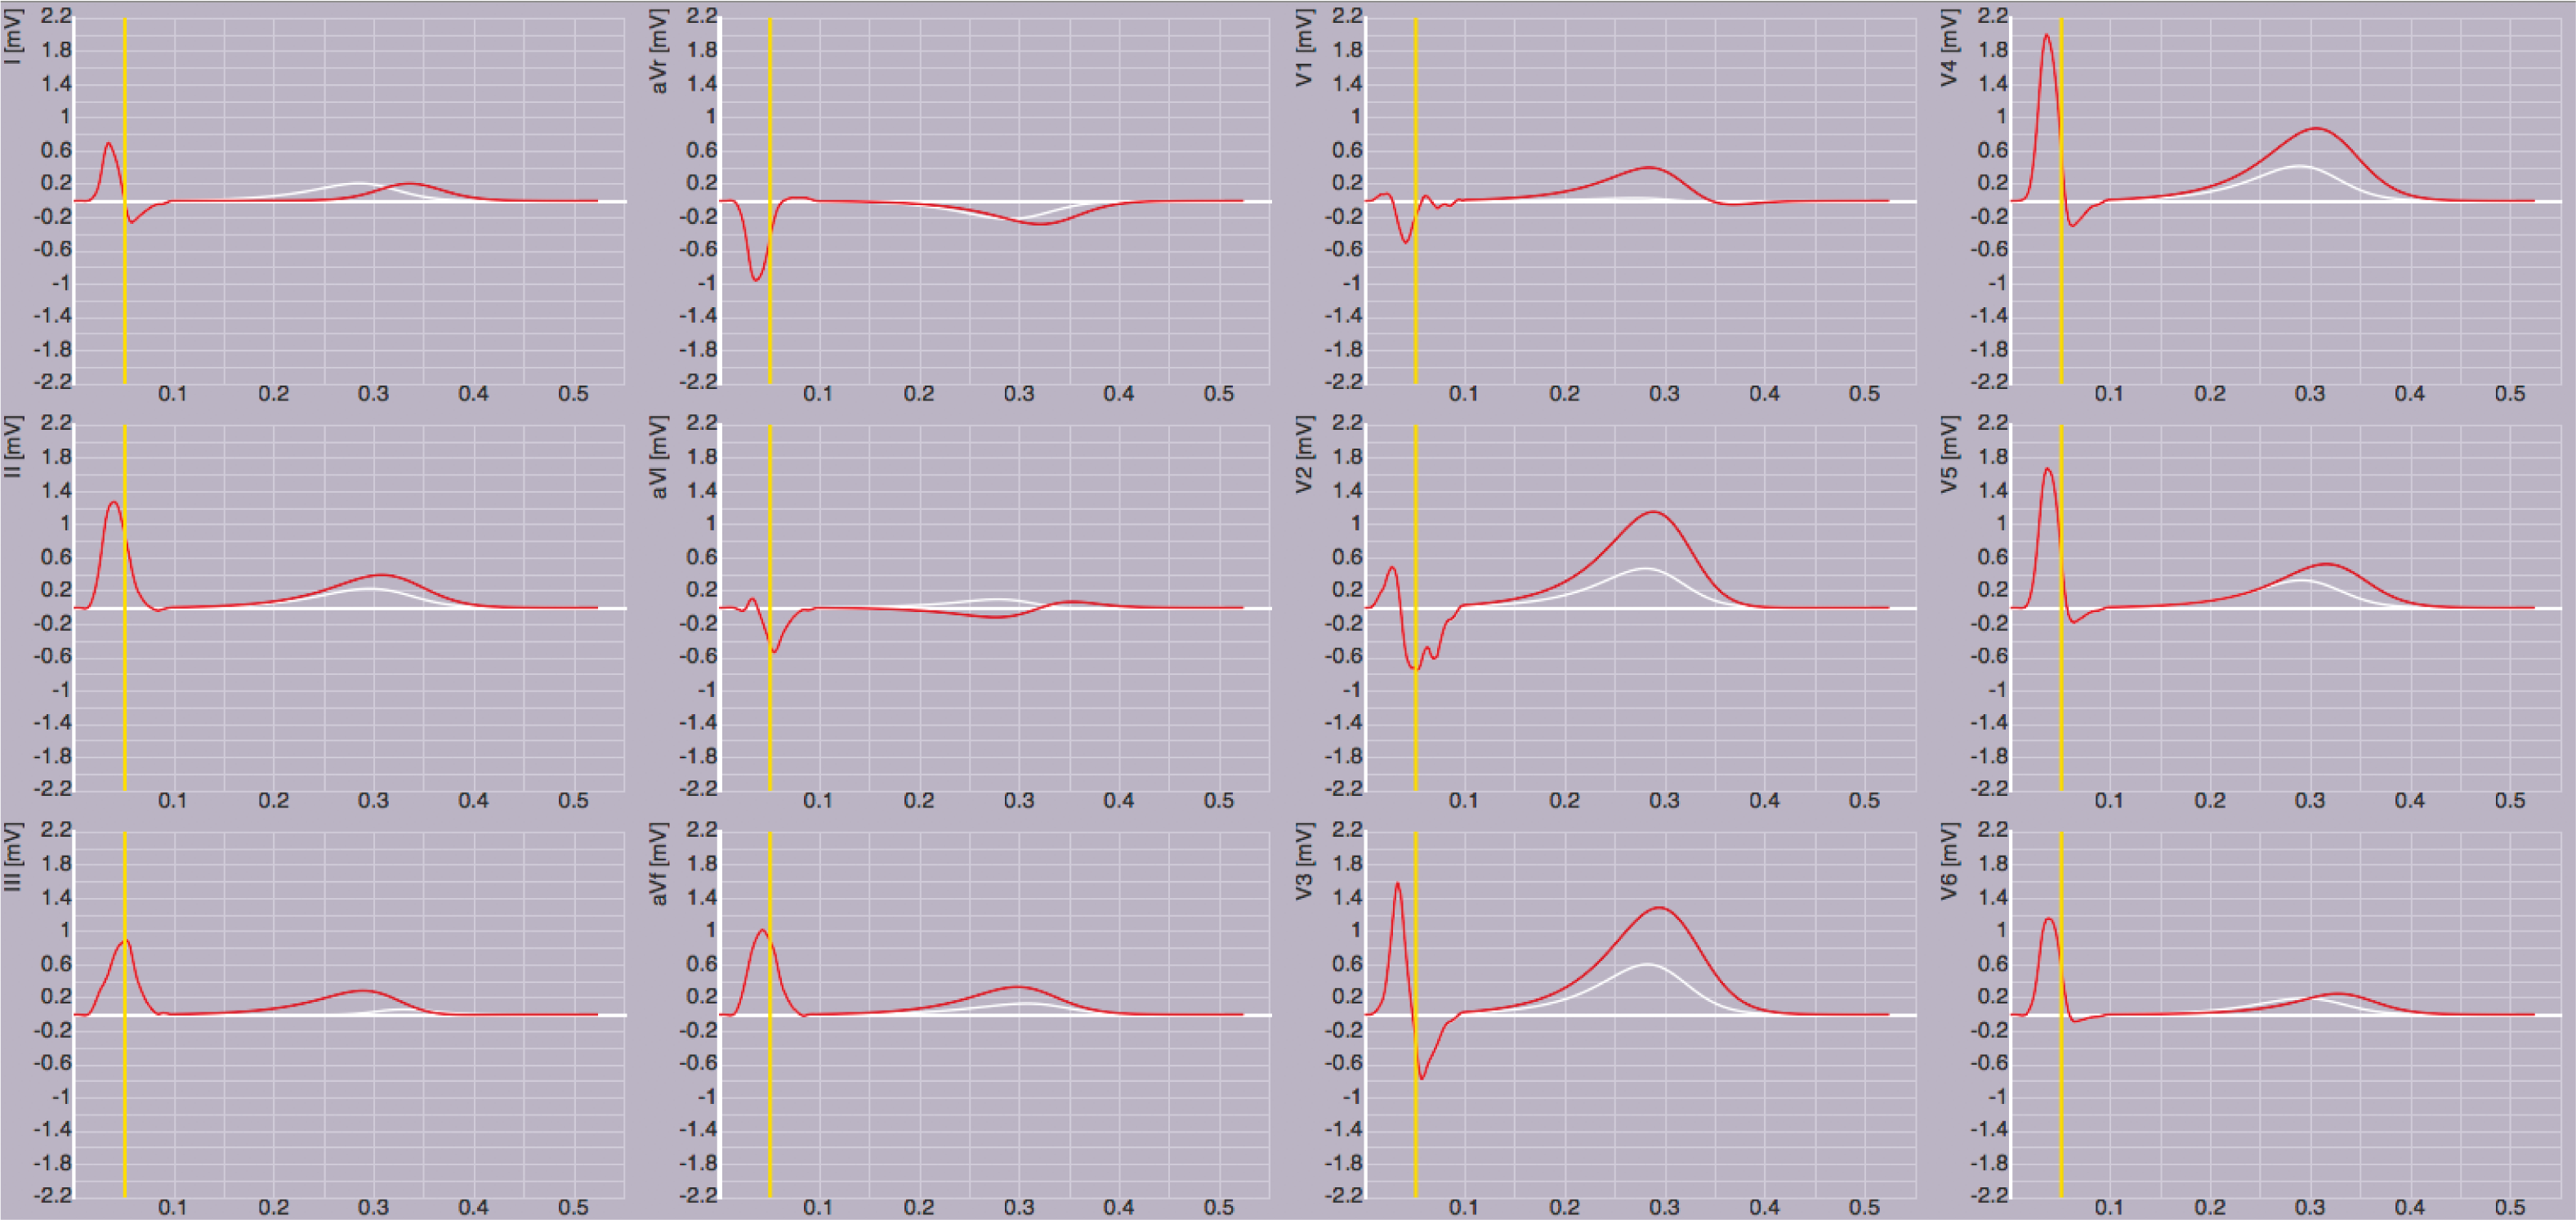
\includegraphics[width=.95\linewidth]{Figures/2_2_25ecg.png}
		\caption{}
		
	\end{subfigure}
	\caption{The ARI map (a), modified action potential (b), and resultant ECG (c) showing the results of prolonging the left ventricular action potential duration by roughly 25\%.}
	\label{2_2_25}
\end{figure}

\begin{figure}[H]
	\begin{subfigure}{.5\textwidth}
		\centering
		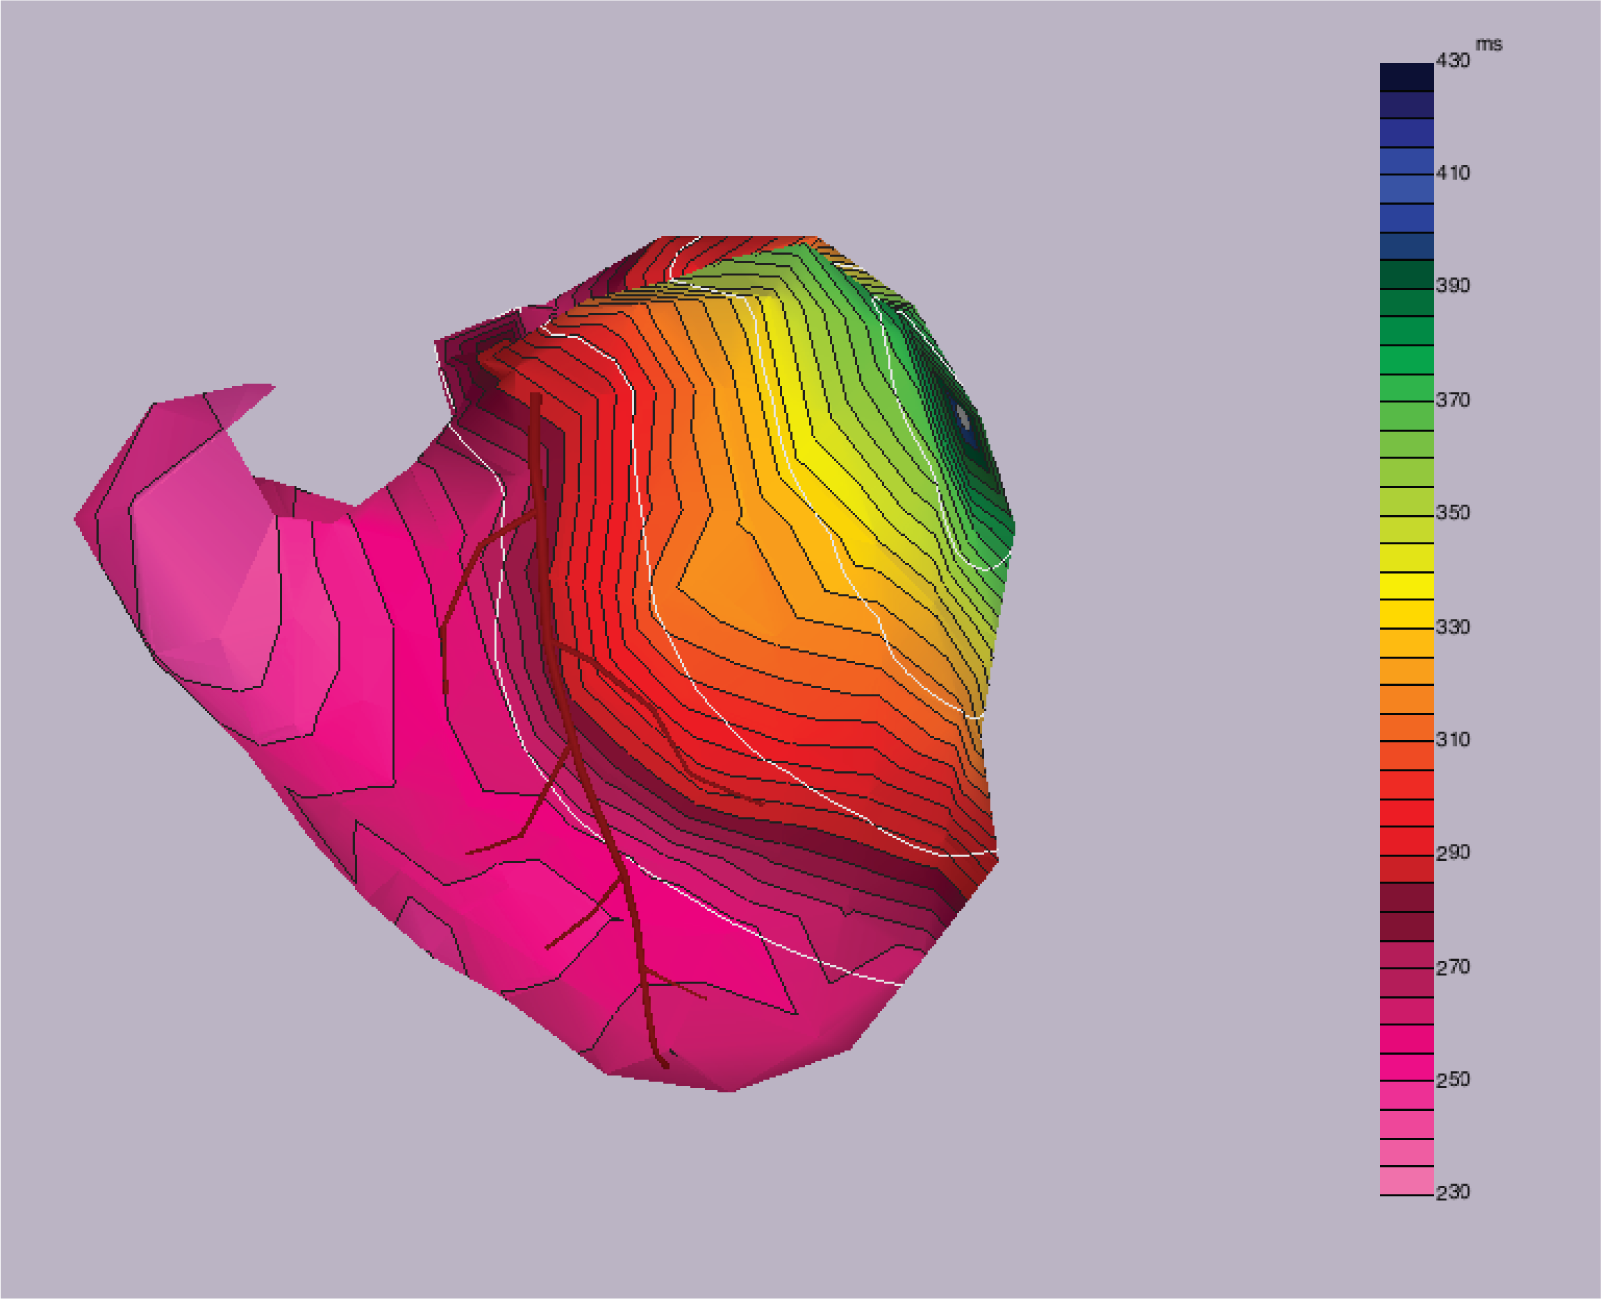
\includegraphics[width=.95\linewidth]{Figures/2_2_50ARI.png}
		\caption{}
		
	\end{subfigure}%
	\begin{subfigure}{.5\textwidth}
		\centering
		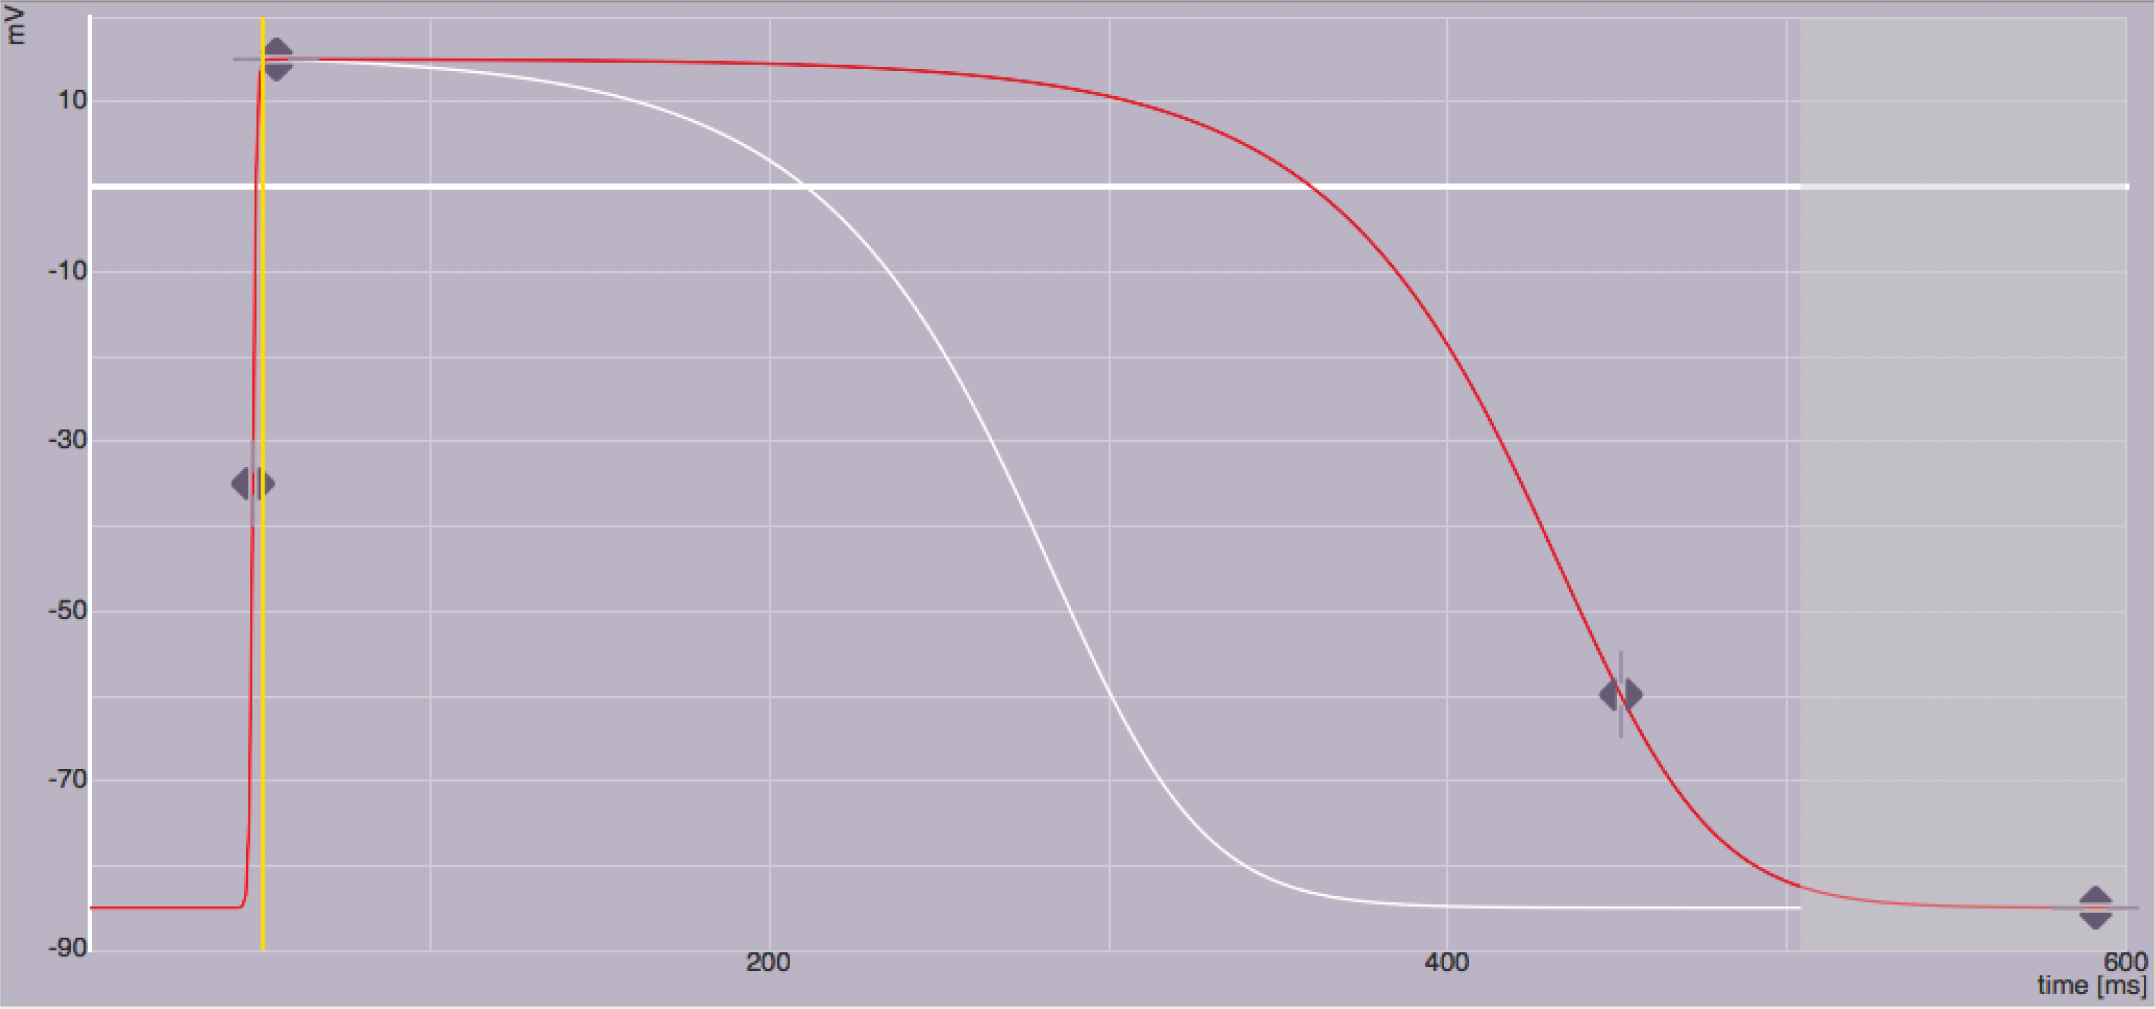
\includegraphics[width=.95\linewidth]{Figures/2_2_50actionpotential.png}
		\caption{}
		
	\end{subfigure}%
	\\
	\begin{subfigure}{.95\textwidth}
		\centering
		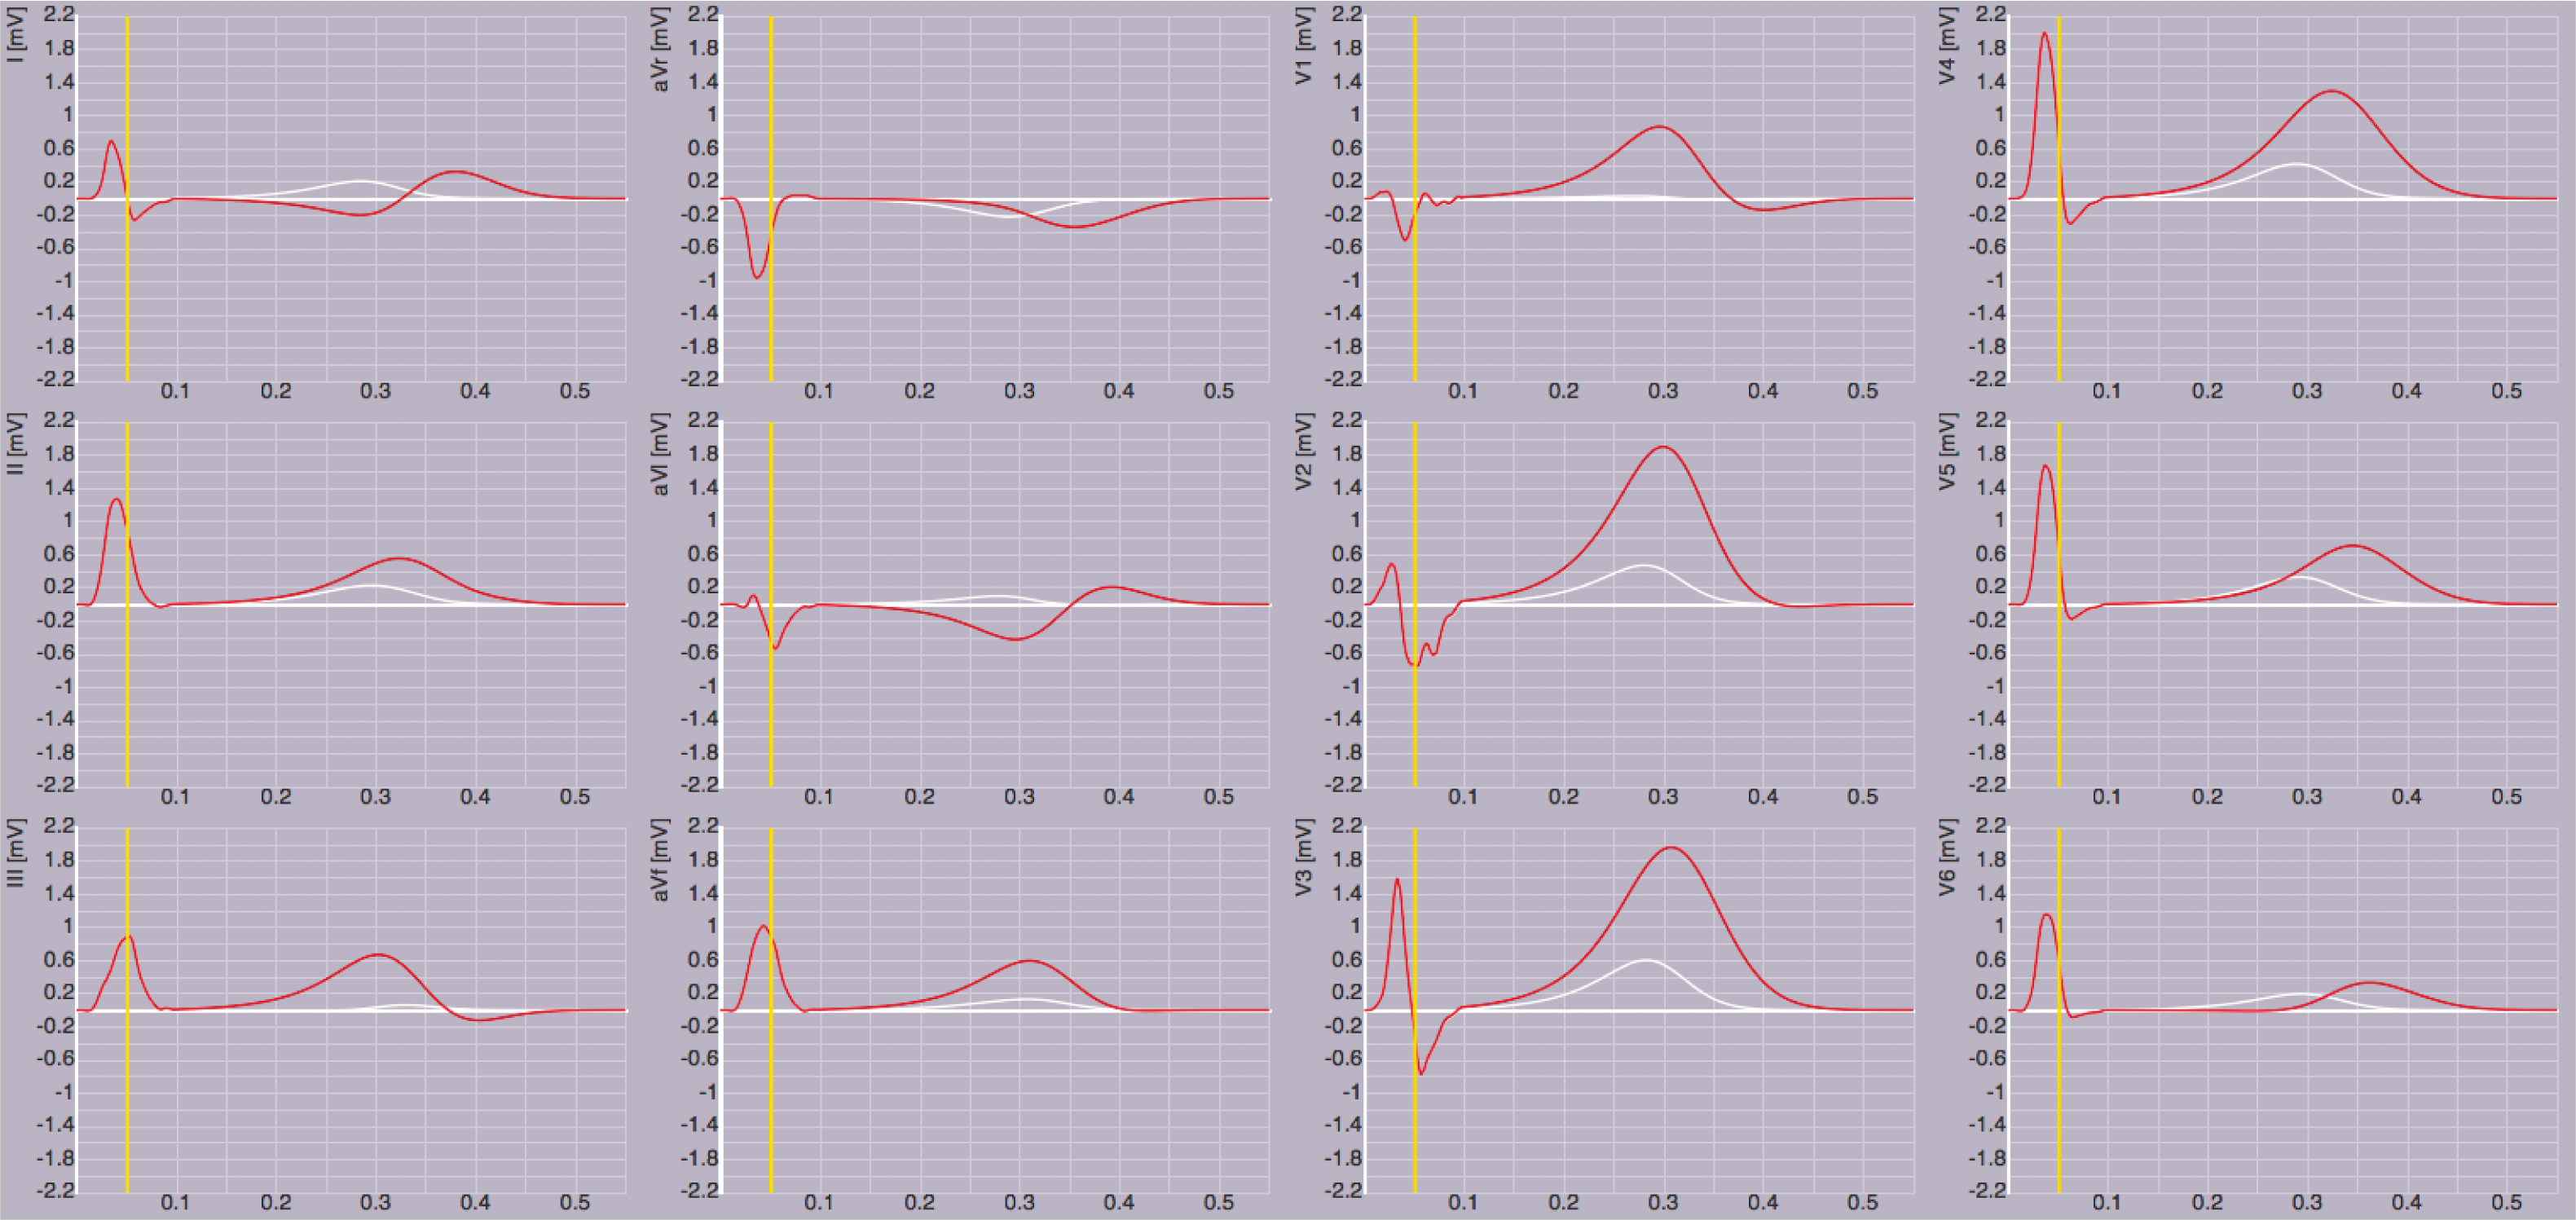
\includegraphics[width=.95\linewidth]{Figures/2_2_50ecg.png}
		\caption{}
		
	\end{subfigure}
	\caption{The ARI map (a), modified action potential (b), and resultant ECG (c) showing the results of prolonging the left ventricular action potential duration by roughly 50\%.}
	\label{2_2_50}
\end{figure}

\subsection{2.3: }
The activation times from my adjustment to mimic left bundle branch along with the associated ECG, and the action potential of the node at the farthest point of the left ventricular free wall is shown in Figure~\ref{2_3}. As can be seen there is a gradient of slower activation that travels from the right ventricle, which activates normally, towards the left ventricular free wall, as would be expected in left bundle branch block. The most distinctive changes to note are widening of the QRS complex, changes in QRS morphology, and changes in T wave morphology (I tried my best to also delay repolaization evenly as I changed activation, however this was difficult and for this reason I will not make much analysis of the T wave changes as they are likely partially artifact due to my inability to homogeneously delay the entire action potential int he left free wall). QRS broadening is to be expected as it takes more time for the ventricles to depolarize. Additionally on Lead I we see a morphology shift. Initially the QRS was positive then negative, as the left ventricular activation (which aligns mostly parallel with lead I) came first and the end of right ventricular activation (which has a wavefront direction mostly antiparallel to lead I) came second. Now with a delayed ventricular activation there is first a negative deflection as the right ventricle activates first then a broad and large positive deflection as the left ventricle slowly depolarizes. The increased amplitude is likely due to the lack of destructive overlap between recording of different activation wavefronts because by the time the left ventricle is depoalrizing that is the only wavefront on the heart. As far as diagnosing this condition based on the ECG, I would use the precordial leads such as V3 in this case. V3 i snear the intraventricular septum and picks up activity from both ventricles as they depolarize. Thus its QRS shows large positive and negative deflections normally, positive when the wave is moving to the right (right ventricular depolarization) and negative when the wave moves to the left (left ventricular depolarization). In this case of left bundle branch there is a very slight positive deflection as the right ventricle activates but it is quickly overtaken by the massive and slow activating wavefront of the right ventricle. This is reflected in an almost completely negative QRS deflection on this lead and a broad QRS. This feature suggests that the activation takes a long time and spends most of its time moving away from V3, and therefor towards the left ventricle. This suggests a slowed and delayed left ventricular activation, indicative of left bundle branch block.

\begin{figure}[H]
	\begin{subfigure}{.5\textwidth}
		\centering
		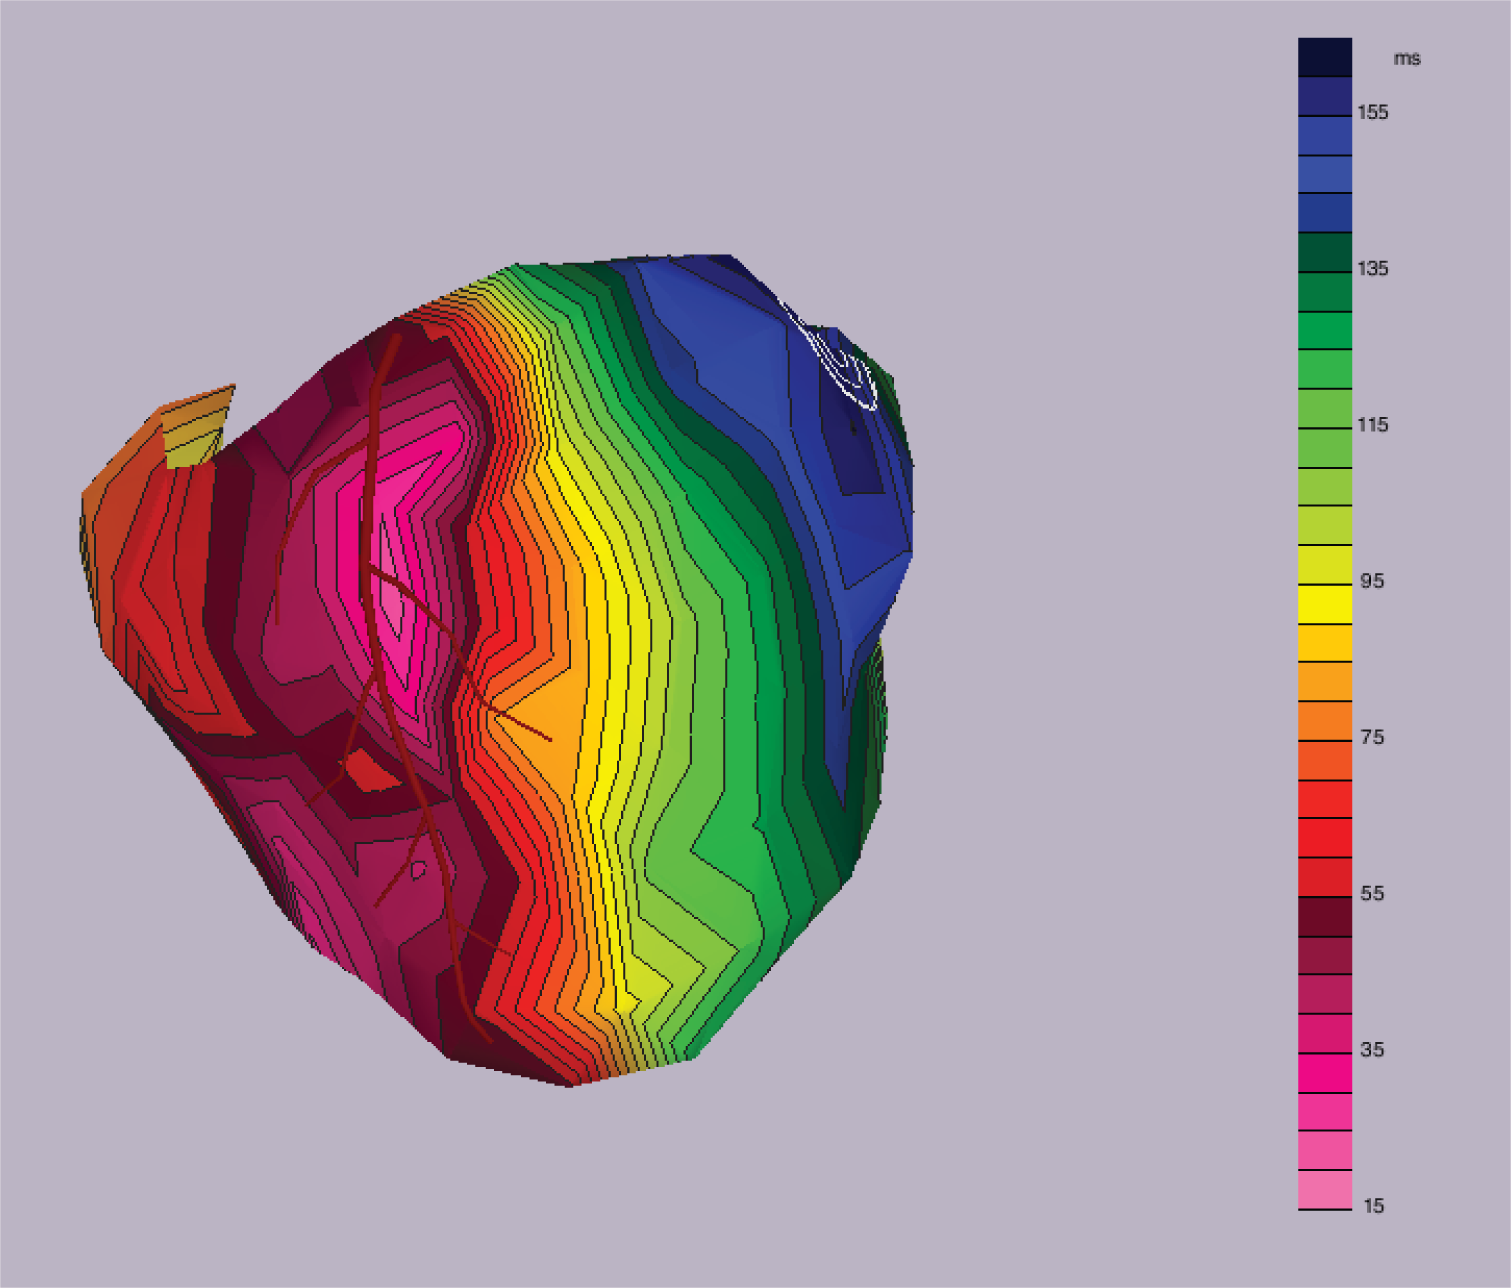
\includegraphics[width=.95\linewidth]{Figures/2_3_actTimes.png}
		\caption{}
		
	\end{subfigure}%
	\begin{subfigure}{.5\textwidth}
		\centering
		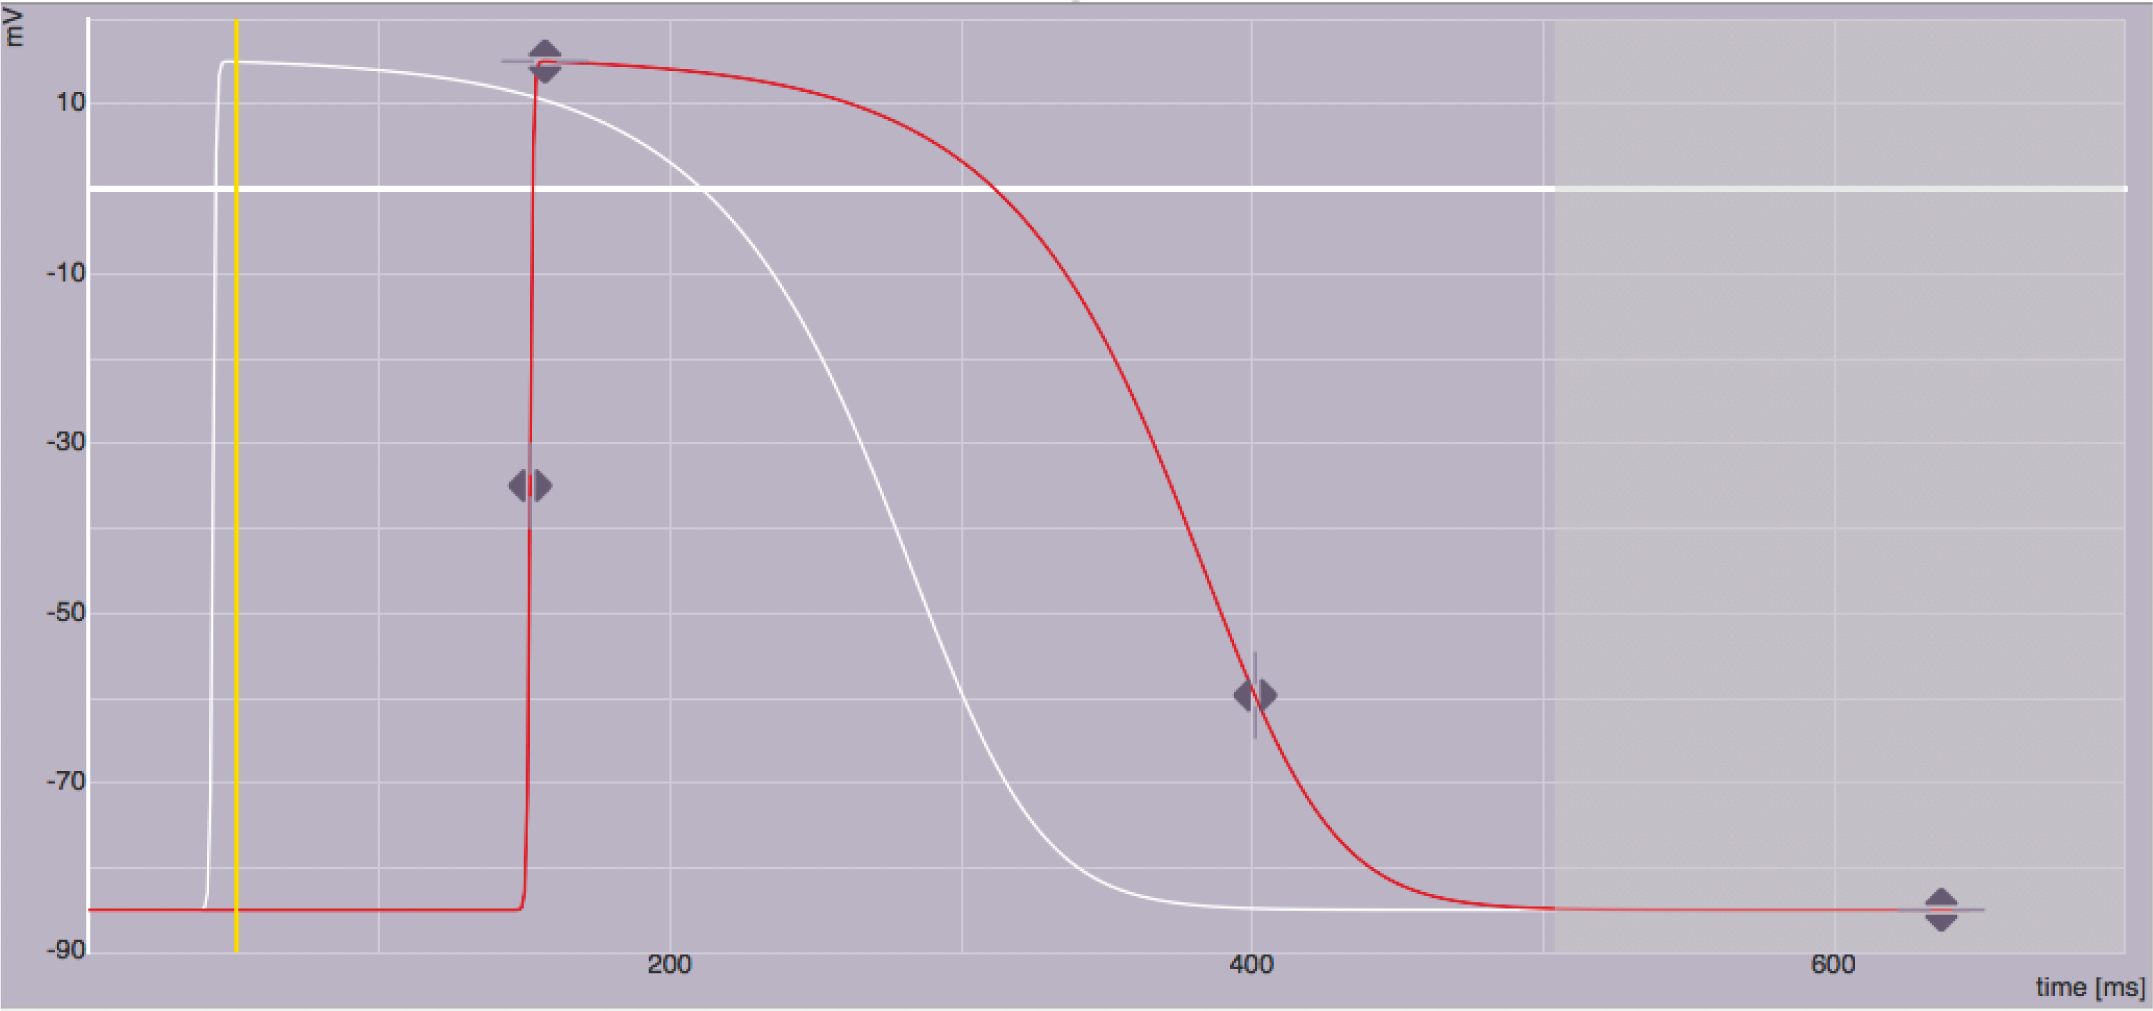
\includegraphics[width=.95\linewidth]{Figures/2_3_actionPotential.png}
		\caption{}
		
	\end{subfigure}%
	\\
	\begin{subfigure}{.95\textwidth}
		\centering
		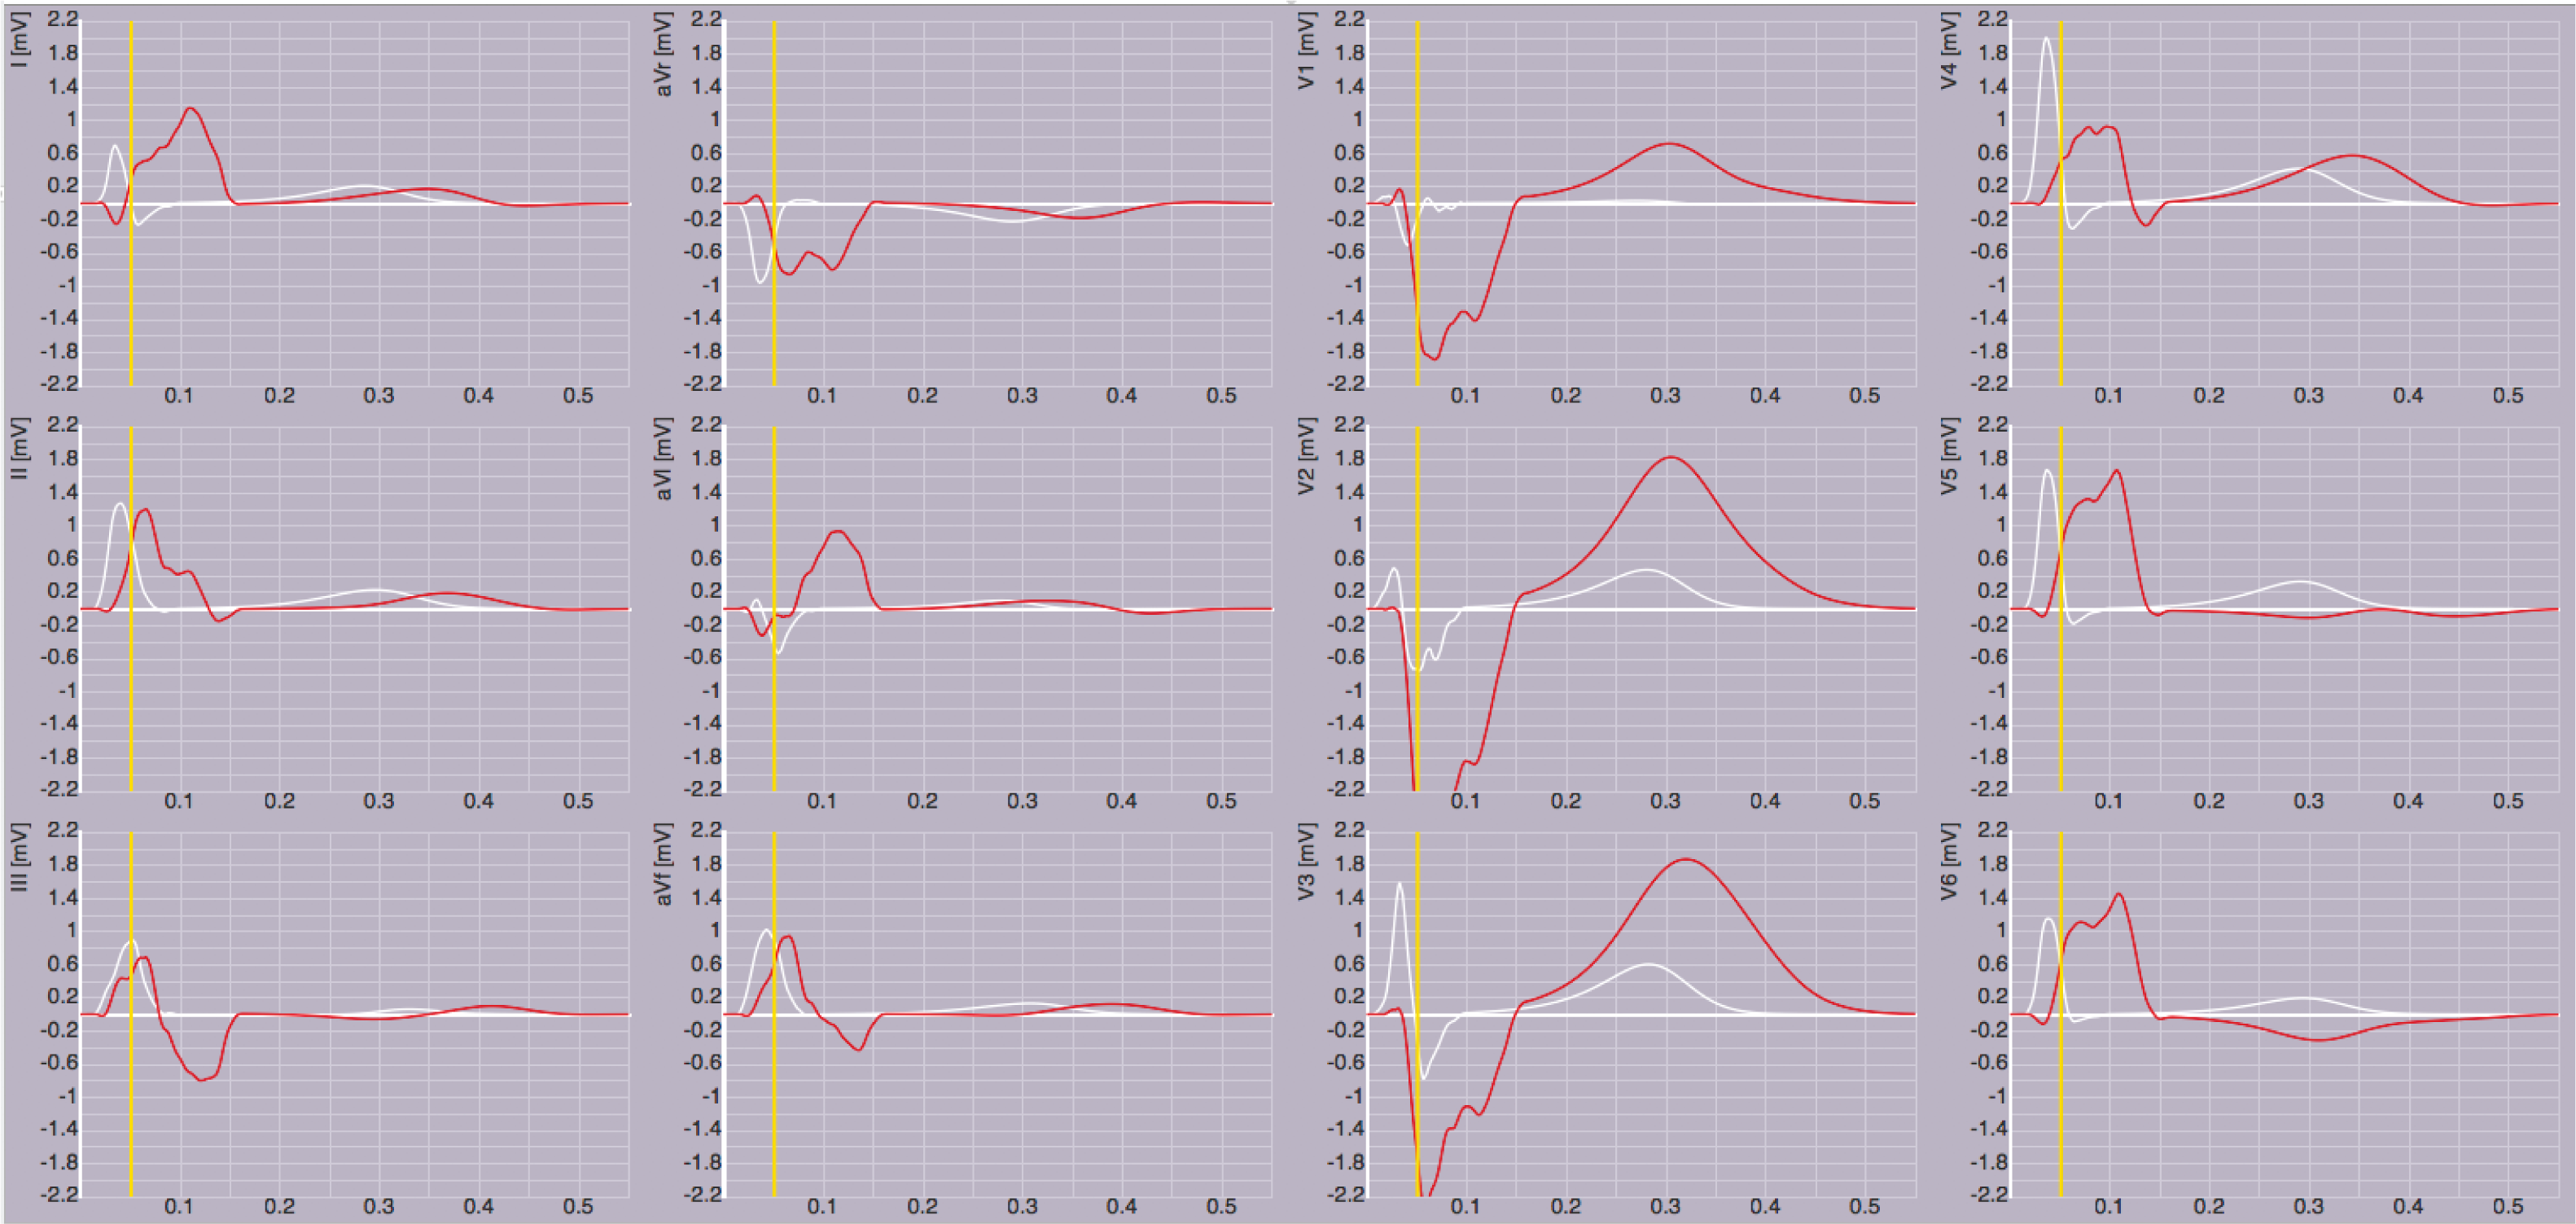
\includegraphics[width=.95\linewidth]{Figures/2_3_ecg.png}
		\caption{}
		
	\end{subfigure}
	\caption{The activation map (a), modified action potential (b), and resultant ECG (c) showing the results of simulating left bundle branch block by delaying activation time of left ventricular nodes.}
	\label{2_3}
\end{figure}

\section{Discussion and Conclusions}


Clearly the ECGSim tool demonstrates the practicality and flexibility of a simulation tool for the investigation of the effects of different cardiac source behaviors and conditions on the resulting body surface ECGs. This simulation environment has the advantage of being free, quick, and flexible. Using this tool researchers can vary several parameters that are impractical or impossible to access during even a large animal or cell culture experimental preparation, such as directly modifying the action potentials of cardiac tissue. This unparalleled level of control allows for very specific and detailed analysis to be performed on a scale that is otherwise impossible. Without such a tool, experiments to replicate these kinds of modifications would require large amounts of experimental tools, expertise, and a lot of funding. Using this simulation tool I was able to quickly assess the effects of changing characteristic features of the heart's electrical activity, and directly observing the consequences on ECG and body surface map recordings. I conclude that this tool is extraordinarily well suited for teaching clinicians, scientists, and generally anyone who is interested about how the electrical activity of the heart manifests on the torso, and how changes to htat electrical activity also manifest.

 However, simulations do have downsides. One obvious shortfall of ECGSim is the lack of atria in the model. Without these the ECG lack the characteristic P wave, and physiological conditions having to do with atrial activity, and ventricular atrial interplay cannot be assessed.  Additionally all models make simplifying assumptions in order to make them computationally feasible. This however limits their translatability to real physiology as the the model does not fully represent physiological function. For example the ECGSim geometries do not allow for changes at a cellular scale nor do they model propagation of activation in the heart or the consequences of tissue heterogeneity such as scar tissue. These limitations prevent analysis of changes to parameters in these areas, and thus limit the scope of the simulation's use.



%%%%%%%%%%%%%%%%%% Correct Bibliography Style

\bibliography{d:/Users/Jake/Documents/library}
\bibliographystyle{ieeetr}


\end{document}








